\documentclass[11pt,a4paper]{article}
\usepackage[top=1.2cm, bottom=1.8cm, left=1.8cm, right=1.8cm]{geometry}

\usepackage[title]{appendix}
\usepackage{float}
\usepackage{subfig}
\usepackage[singlelinecheck=false]{caption}
\usepackage{graphicx}
\usepackage{listings}
\usepackage{color}
\usepackage[utf8]{inputenc}
\usepackage{minted}
\usepackage{amsmath}
\usepackage{enumitem}
\usepackage{siunitx}

\usepackage[style=authoryear, backend=biber]{biblatex}
\addbibresource{main.bib}
\DeclareMathOperator*{\argmin}{arg\,min}
\DeclareMathOperator*{\argmax}{arg\,max}

\title{COMP6202: Assignment 2}
\author{
David Jones \\
dsj1n15@soton.ac.uk, ID: 27549836}
\date{}
\setlength{\intextsep}{1mm}

\begin{document}

\maketitle

\section{Introduction}
\textbf{Paper Re-Implemented:}\\
Coevolutionary Dynamics in a Minimal Substrate \parencite{Watson:2001}

\subsection{Experiments}
The experiments described by \cite{Watson:2001} are designed to demonstrate potential issues in co-evolutionary genetic algorithm (GA) implementations; usually stemming from a difference in the \textit{subjective fitness}  of an individual and its \textit{objective fitness} ($f_\text{obj}(i) \neq f_\text{subj}(i)$). The former being the fitness as perceived by an individual co-evolving with other individuals, and the latter being the individual's actual fitness assessed via a fixed metric. The use of a subjective metric is key in GA applications as often an objective metric is not available. Although this provides benefits such as open-endedness (every time an individual improves it is the new target to beat), it can pose issues including:
\begin{enumerate}[label=\Alph*]
    \item Disengagement: If all individuals in one population become able to beat all individuals in the other, there is a loss of gradient information and performance may drift without guidance.
    \item Over-Specialisation: Where an individual has multiple \textit{traits}, other individuals may exploit a single one, leaving other traits undeveloped. These individuals are not generalised and may not learn the task at hand.
    \item `Relativism': Co-adapting individuals are relatively scored against each other so $\text{P}_\text{subj}(a, b)$ may be equal if both $a$ and $b$ are good or if both $a$ and $b$ are bad; giving no selection incentive to be good.
\end{enumerate}
In complex scenarios it is hard to identify when these scenarios occur so \cite{Watson:2001} prove these phenomena on a ``minimal substrate''. Specifically, the problem of maximising the number of `1's in a fixed length bitstring or vector of bitstrings. This has a quantifiable objective fitness for external assessment: $f(i)=ones(i)$. It is a reasonable assumption that if pre-mentioned failures occur on this simple example, they are possible in complex examples.\\

% ($\text{P}_\text{obj}(a, b)$)
% ($\text{P}_\text{subj}(a, b)$)


\subsection{Implementation}
Reimplementation of the original paper was done in Python and can be found in Appendix \ref{sec:codebase}. Individuals are implemented as a vector of traits ($i=[t_1, t_2, \dots, t_n]$) where a single trait is a scalar value representing the number of set bits ($t=t_\text{value}=ones(t_\text{bitstring})$). This is simpler  than storing bitstrings with the drawback that crossover cannot be implemented. An individual is defined by the number of bits in each trait ($t_l$) and the number of traits ($t_c$); fully defined this is $i=\{t_c,t_l\}$.
$f_\text{obj}(i)$ is defined as the sum of \textit{ones} across all traits ($\sum^{t_c}_{n=1}ones(i(n))$. To allow assessment in a GA $f_\text{subj}$ is defined as: $f(a, S)$ where $a$ is an individual and $S$ is a sample of the opponent population (with replacement), $|S|=15$ unless stated. Scoring is fully defined by Equation \ref{eq:scoring}. Intransitivity is \textit{false} unless stated.

\begin{equation}
\label{eq:scoring}
\begin{split}
&f(a, S)=\sum^{|S|}_{i=1}\frac{score(a, S_i)}{|S|} \\
&\text{where } score(a,b) = 1 \text{ if } a(d) > b(d), 0 \text{ otherwise} \\
&\text{where } d =
\begin{cases}
    \argmin_d (a, b) = |a(d) - b(d)|& \text{if intransitive}\\
    \argmax_d (a, b) = |a(d) - b(d)|& \text{otherwise}\\
\end{cases}
\end{split}
\end{equation}
The two populations of individuals are defined as $P_A$ and $P_B$; both of size $25$ ($|P|$). Combined, the full GA algorithm is described as: \textbf{assess} the subjective fitness of each population, \textbf{select} $|P|$ individuals based on their fitness, \textbf{mutate} each individual, \textbf{insert} them into a new population, and \textbf{repeat}. This is a description of a generational GA. Selection is implemented as fitness proportionate selection where each individual has probability $p(i)$ of getting selected where $p(i)=\frac{f_\text{subj}(i)}{\sum^n_{j=1}f_\text{subj}(j)}$. This selection occurs  $|P|$ times for each $P_A$ and $P_B$ to form the new populations. Note that as this selection is modelled as a \textit{roulette wheel} the wheel will not \textit{spin} when encountering individuals where $f_\text{subj}(i)=0$. This issue is clearest when all elements have $f_\text{obj}=0$, as $p(P(0))=1$ and $p(P{>0})=0$. This is mitigated by adding a fixed bias that is close to 0 ($b = \num{1e-5}$) to all fitnesses. The mutation operator is defined as each bit in each trait having a chance to set to a new random value (0 or 1). This is implemented on the scalars as the original value having a $0.5\%$ chance of having a $50\%$ chance of decreasing $ones(t)$ times and increasing $t_l - ones(i)$ times. This captures inherit mutation bias that would be present in a bitstring, i.e. a string with more zeros than ones is likely to increase rather than decrease, meaning each trait will drift to $\frac{t_l}{2}$ This bias is key to patterns shown and is demonstrated in Figure \ref{fig:figure_1}. 


\section{Reimplementation Results}
Overall the reimplementation of figures was successful with the expected patterns shown. For objective fitness all raw data points and an average trend line are plotted. For subjective fitness the average score for all individuals in the population is shown.
\subsection{Experiment 1}
\noindent The first experiment is configured to demonstrate disengagement resulting in a loss of gradient. The reproduced figure (Figure \ref{fig:figure_3}) shows this occurring in the form of drifting back to the neutral level during the polarised stages (generations 150-220 and 400-540) -- polarisation can be identified by $f_\text{subj}$ being 0 for one population and 1 for the other. Peaks are not as pronounced as the original, suggesting re-engagement happens quickly, however, as this occurs non-deterministically when the neutral position is approached the result is not considered an anomaly. For this problem disengagement can be fixed by providing a less polarising competition by increasing $|S|$; this is demonstrated in Figure \ref{fig:figure_2}. The clear contrast is that Figure \ref{fig:figure_2} has a steady ascent until the maximum objective $f_\text{obj}$ is reached, whereas this experiment does not reach the maximum due to occasional descents.

\begin{figure}[H]
    \centering
    \begin{tabular}{cc}
    \subfloat[Original \parencite{Watson:2001}]{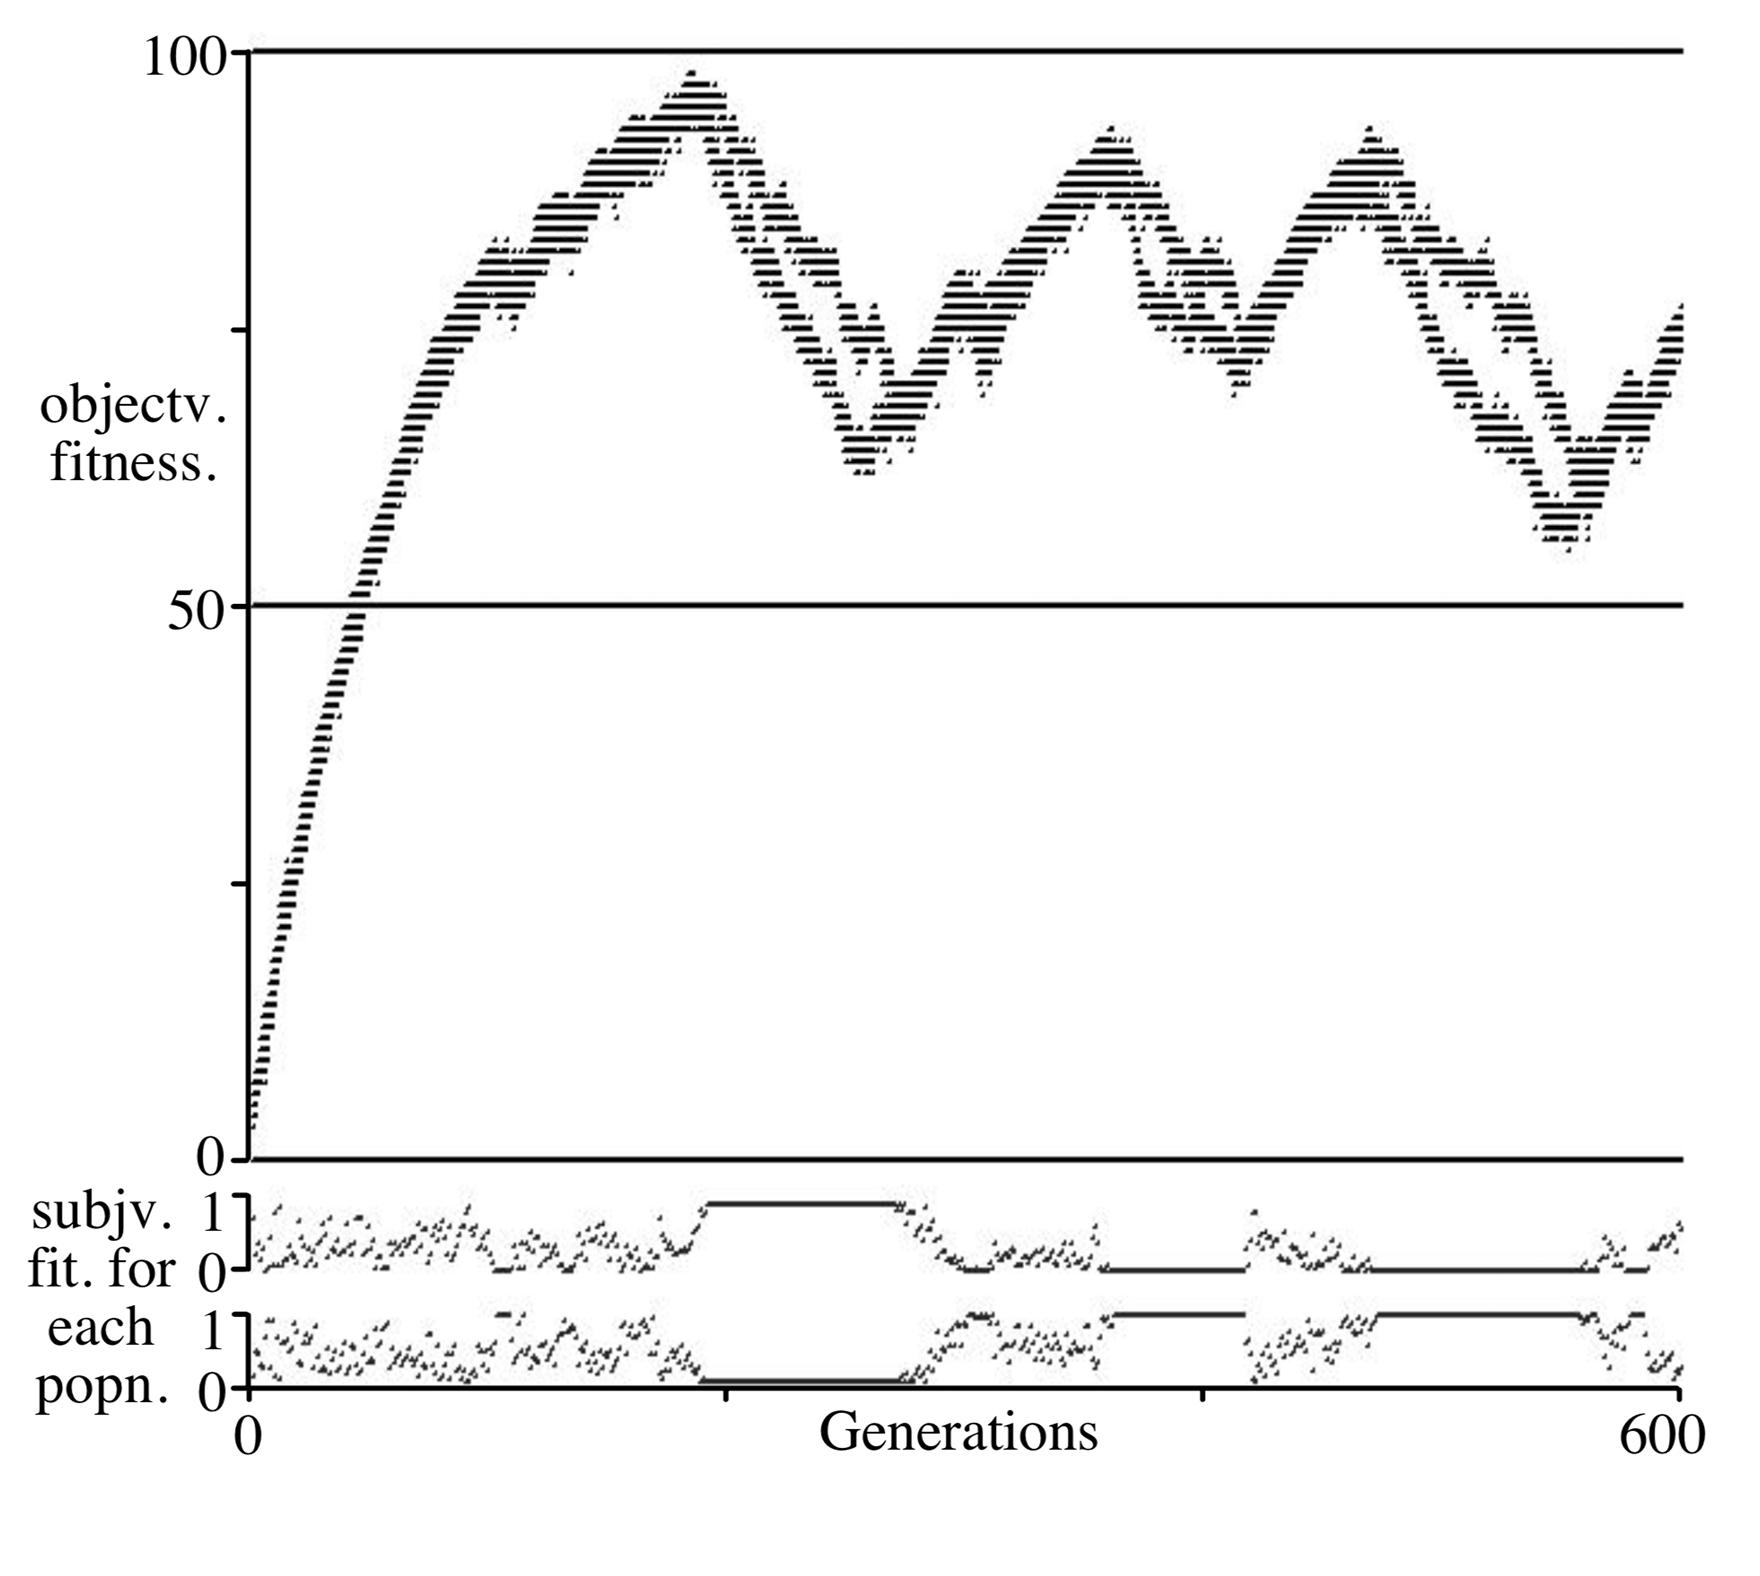
\includegraphics[height=6.5cm]{original/fig3.png}}
    \hspace{1.5mm}
    \subfloat[Reimplementation]{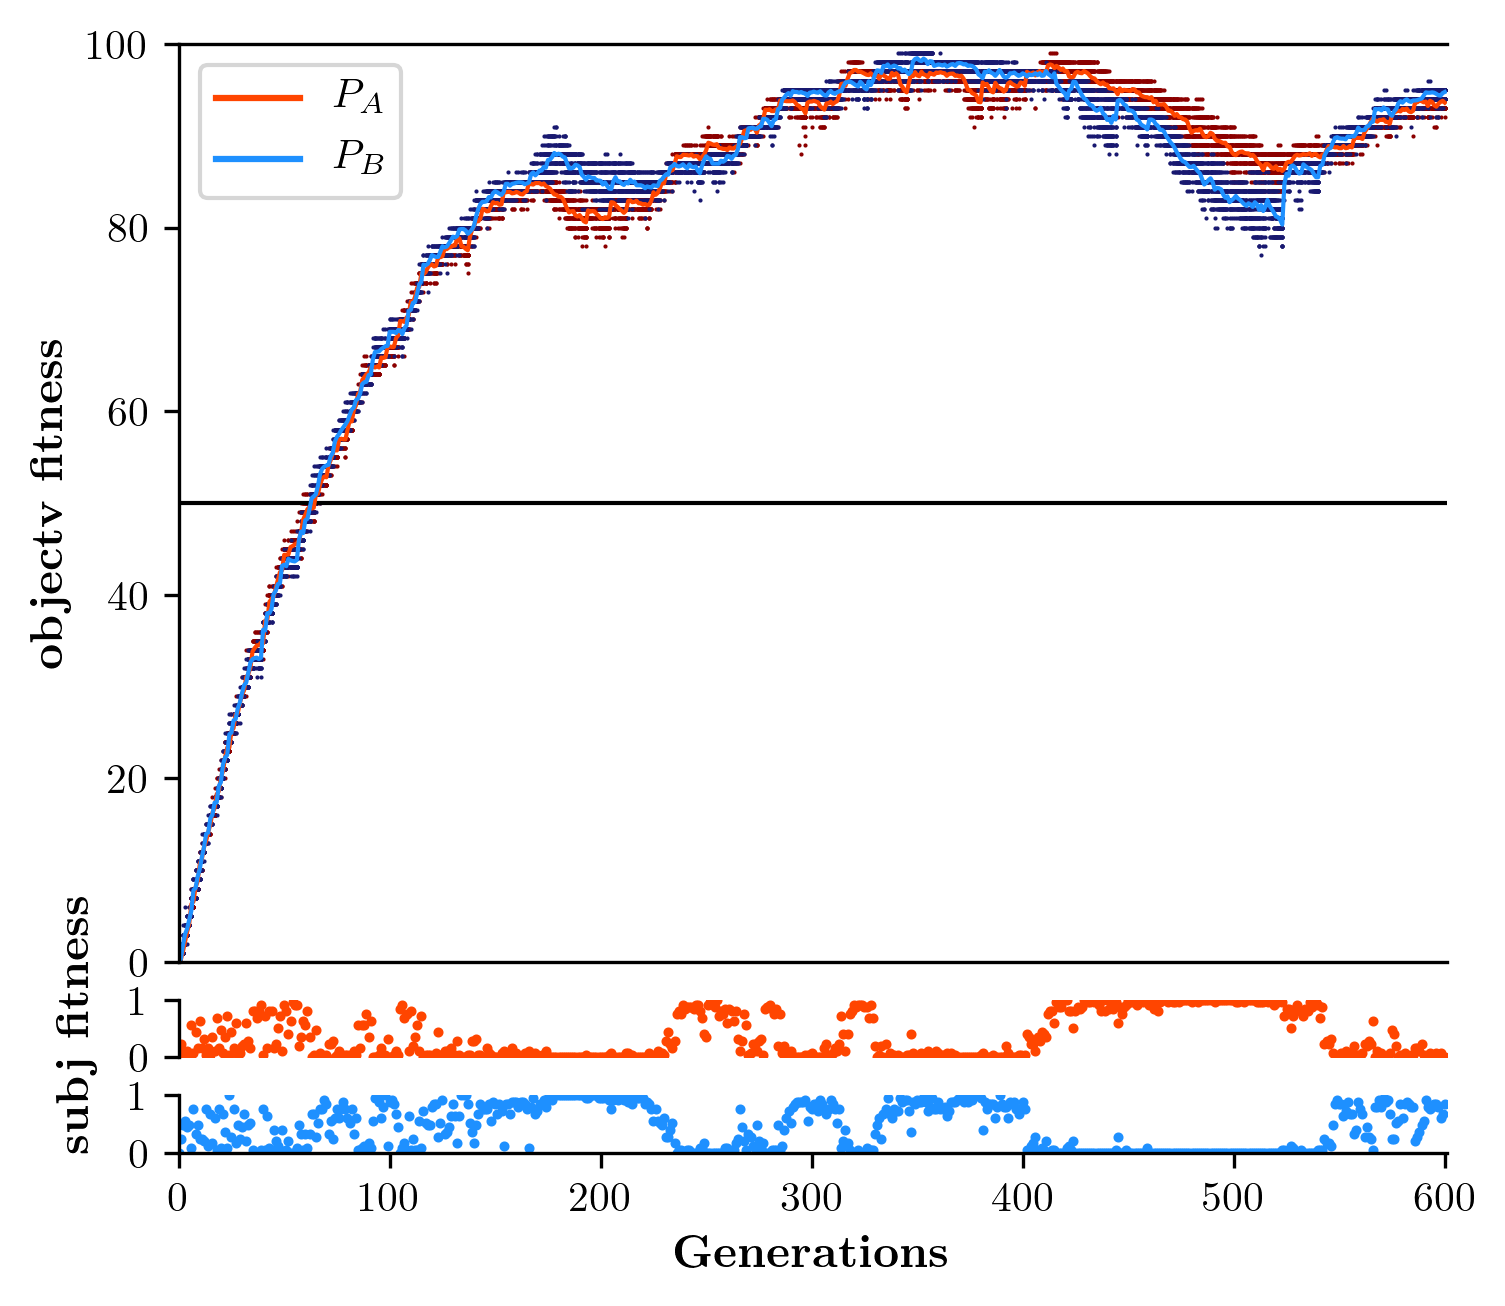
\includegraphics[height=6.5cm]{plots/fig3.png}}
    \end{tabular}
    \caption{$i=\{1,100\}$, $|S|=1$ \textit{(Originally Figure 3)}}
    \label{fig:figure_3}
\end{figure}
\subsection{Experiment 2}
The second experiment concerns monitoring for over specialisation by increasing the number of dimensions in the individual. With intransitivity disabled, Equation \ref{eq:scoring} now applies scoring using the trait with the largest difference. This is implemented in Figure \ref{fig:figure_4} and as expected, unlike Figure \ref{fig:figure_2}, the fitness does not reach 100 due to an inability to maintain traits that are not being assessed as part of fitness assessments. This lack of dominance in all traits means even the elite of both populations is not guaranteed to beat an individual from a new population, i.e. they are overly focussed.

\begin{figure}[H]
    \centering
    \begin{tabular}{cc}
    \subfloat[Original \parencite{Watson:2001}]{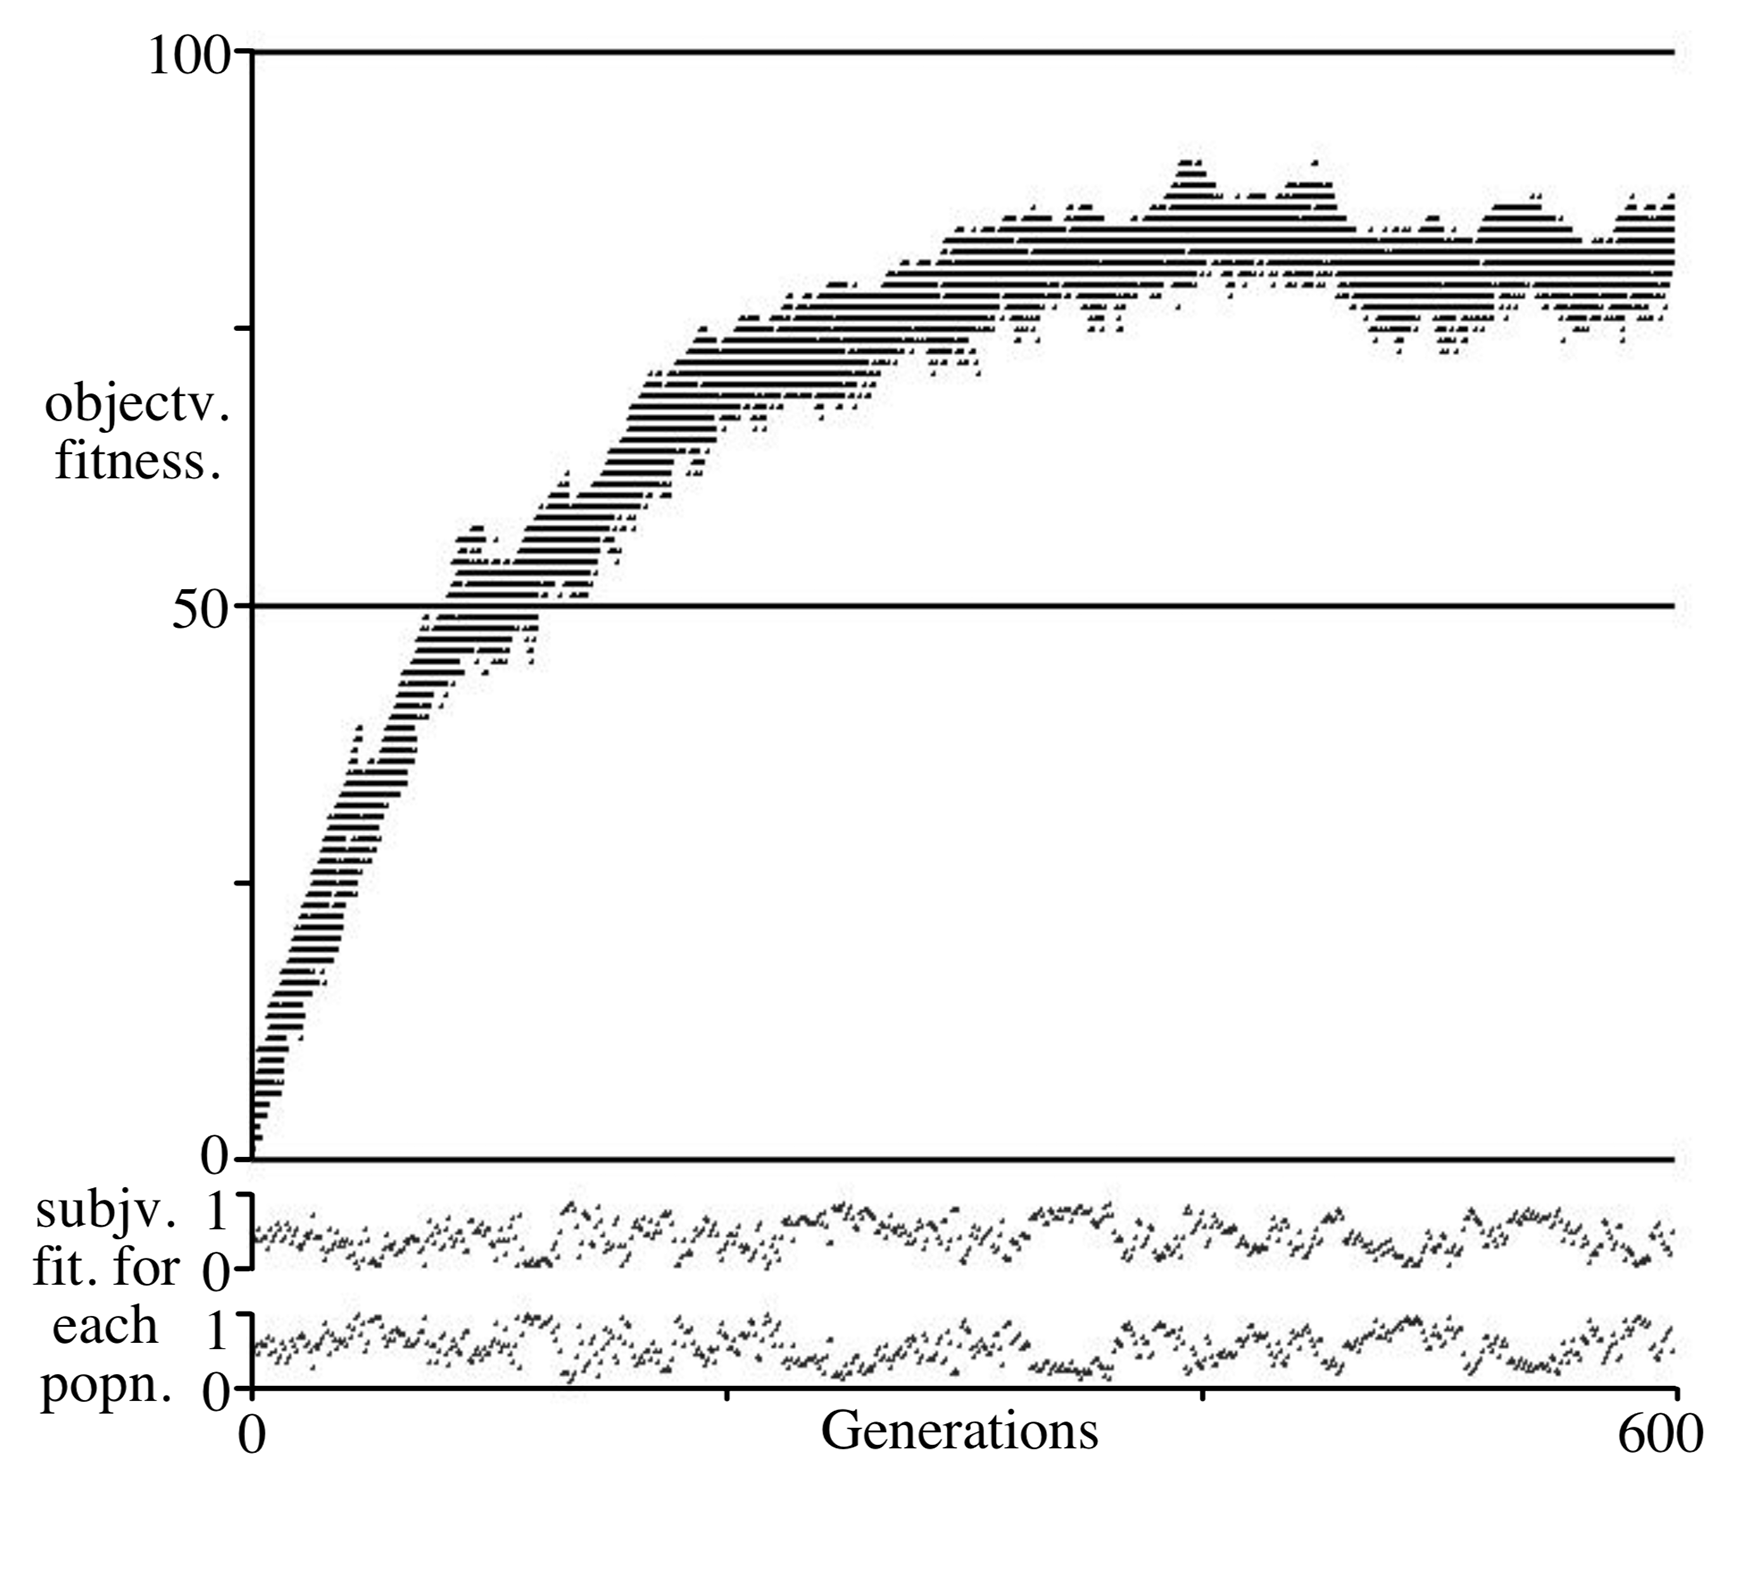
\includegraphics[height=6.5cm]{original/fig4.png}}
    \hspace{1.5mm}
    \subfloat[Reimplementation]{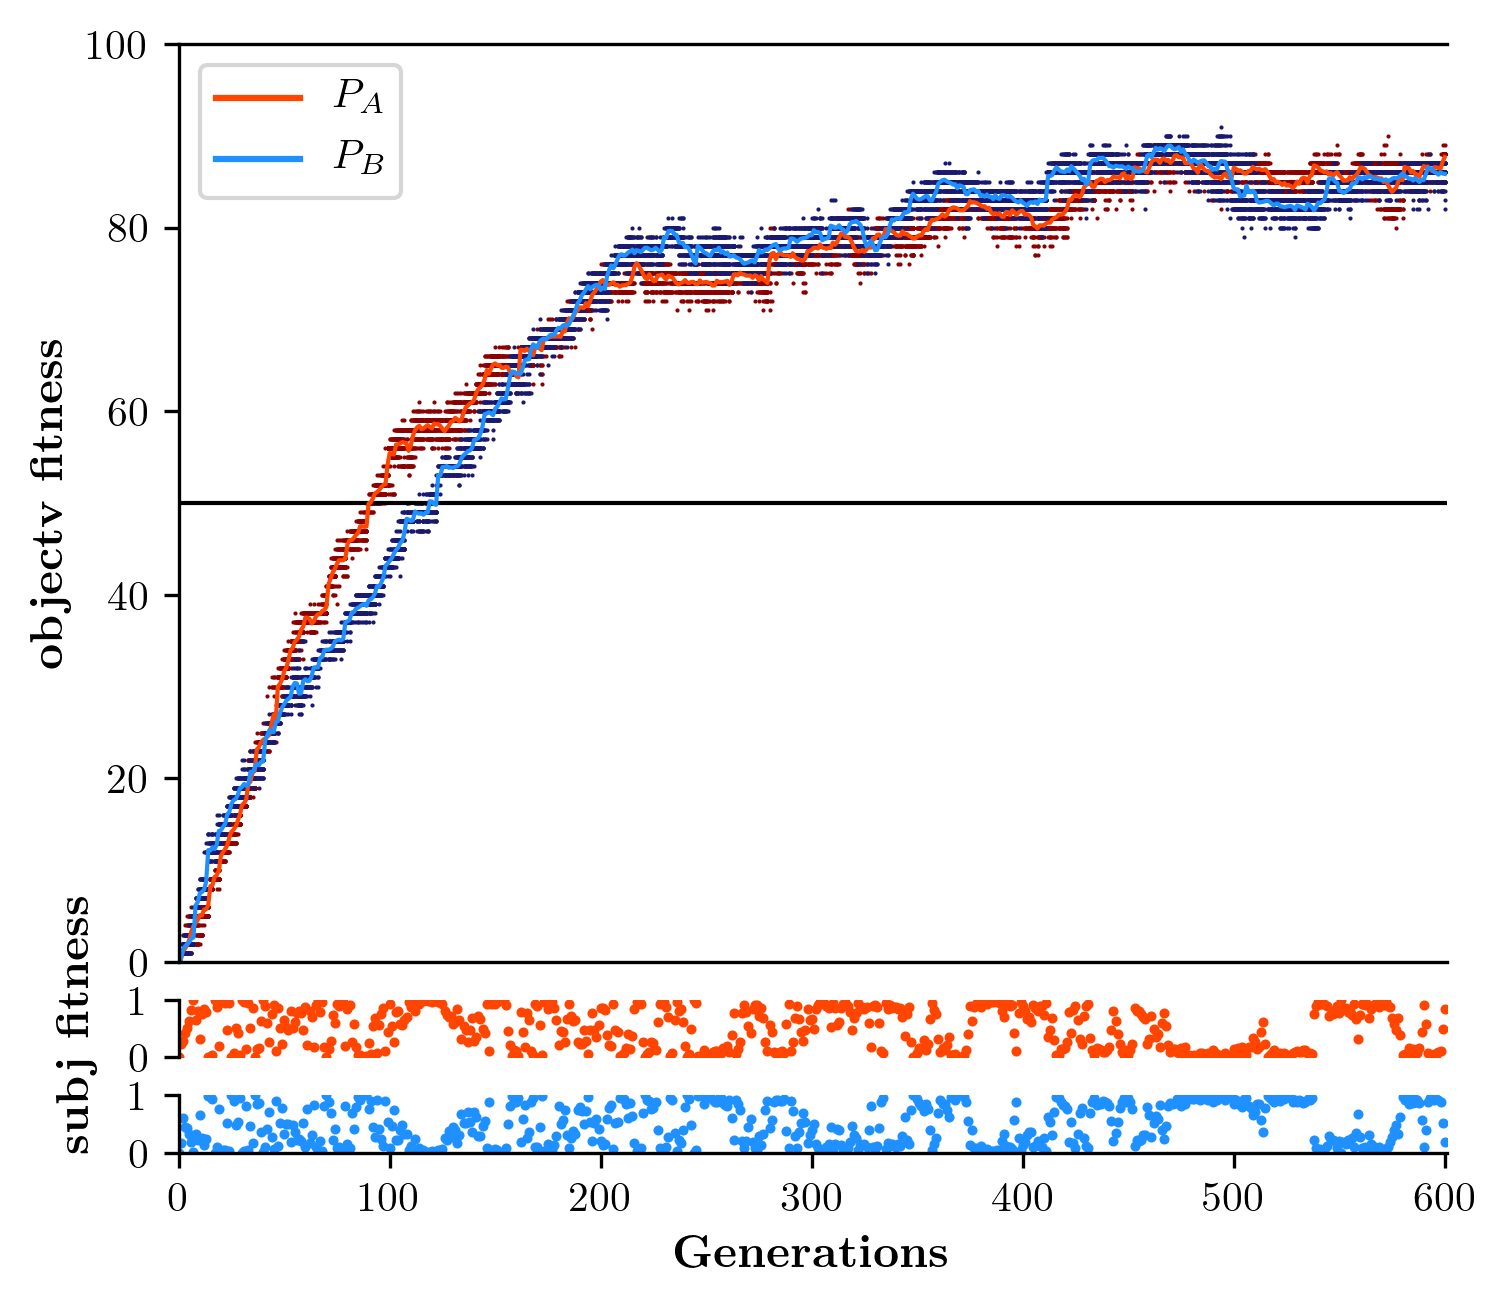
\includegraphics[height=6.5cm]{plots/fig4.png}}
    \end{tabular}
    \caption[]{$i=\{10,10\}$ \textit{(Originally Figure 4)} }
    \label{fig:figure_4}
\end{figure}
\subsection{Experiment 3}
The third experiment is an example of relativism via intransitivity. With intransitivity enabled, Equation \ref{eq:scoring} now applies scoring using the trait with the smallest difference. This is implemented in Figure \ref{fig:figure_5} where the objective score is clearly being driven down away from the mutation bias level (generations 150-250) even more than that in the original paper -- all whilst the subjective score is not polarised. This indicates that $f_\text{subj}$ must be the opposite to $f_\text{obj}$ and indicates an individual would rather lower its overall score to ensure its strongest trait is selected most times; this is a demonstration of cyclic superiority.

\begin{figure}[H]
    \centering
    \begin{tabular}{cc}
    \subfloat[Original \parencite{Watson:2001}]{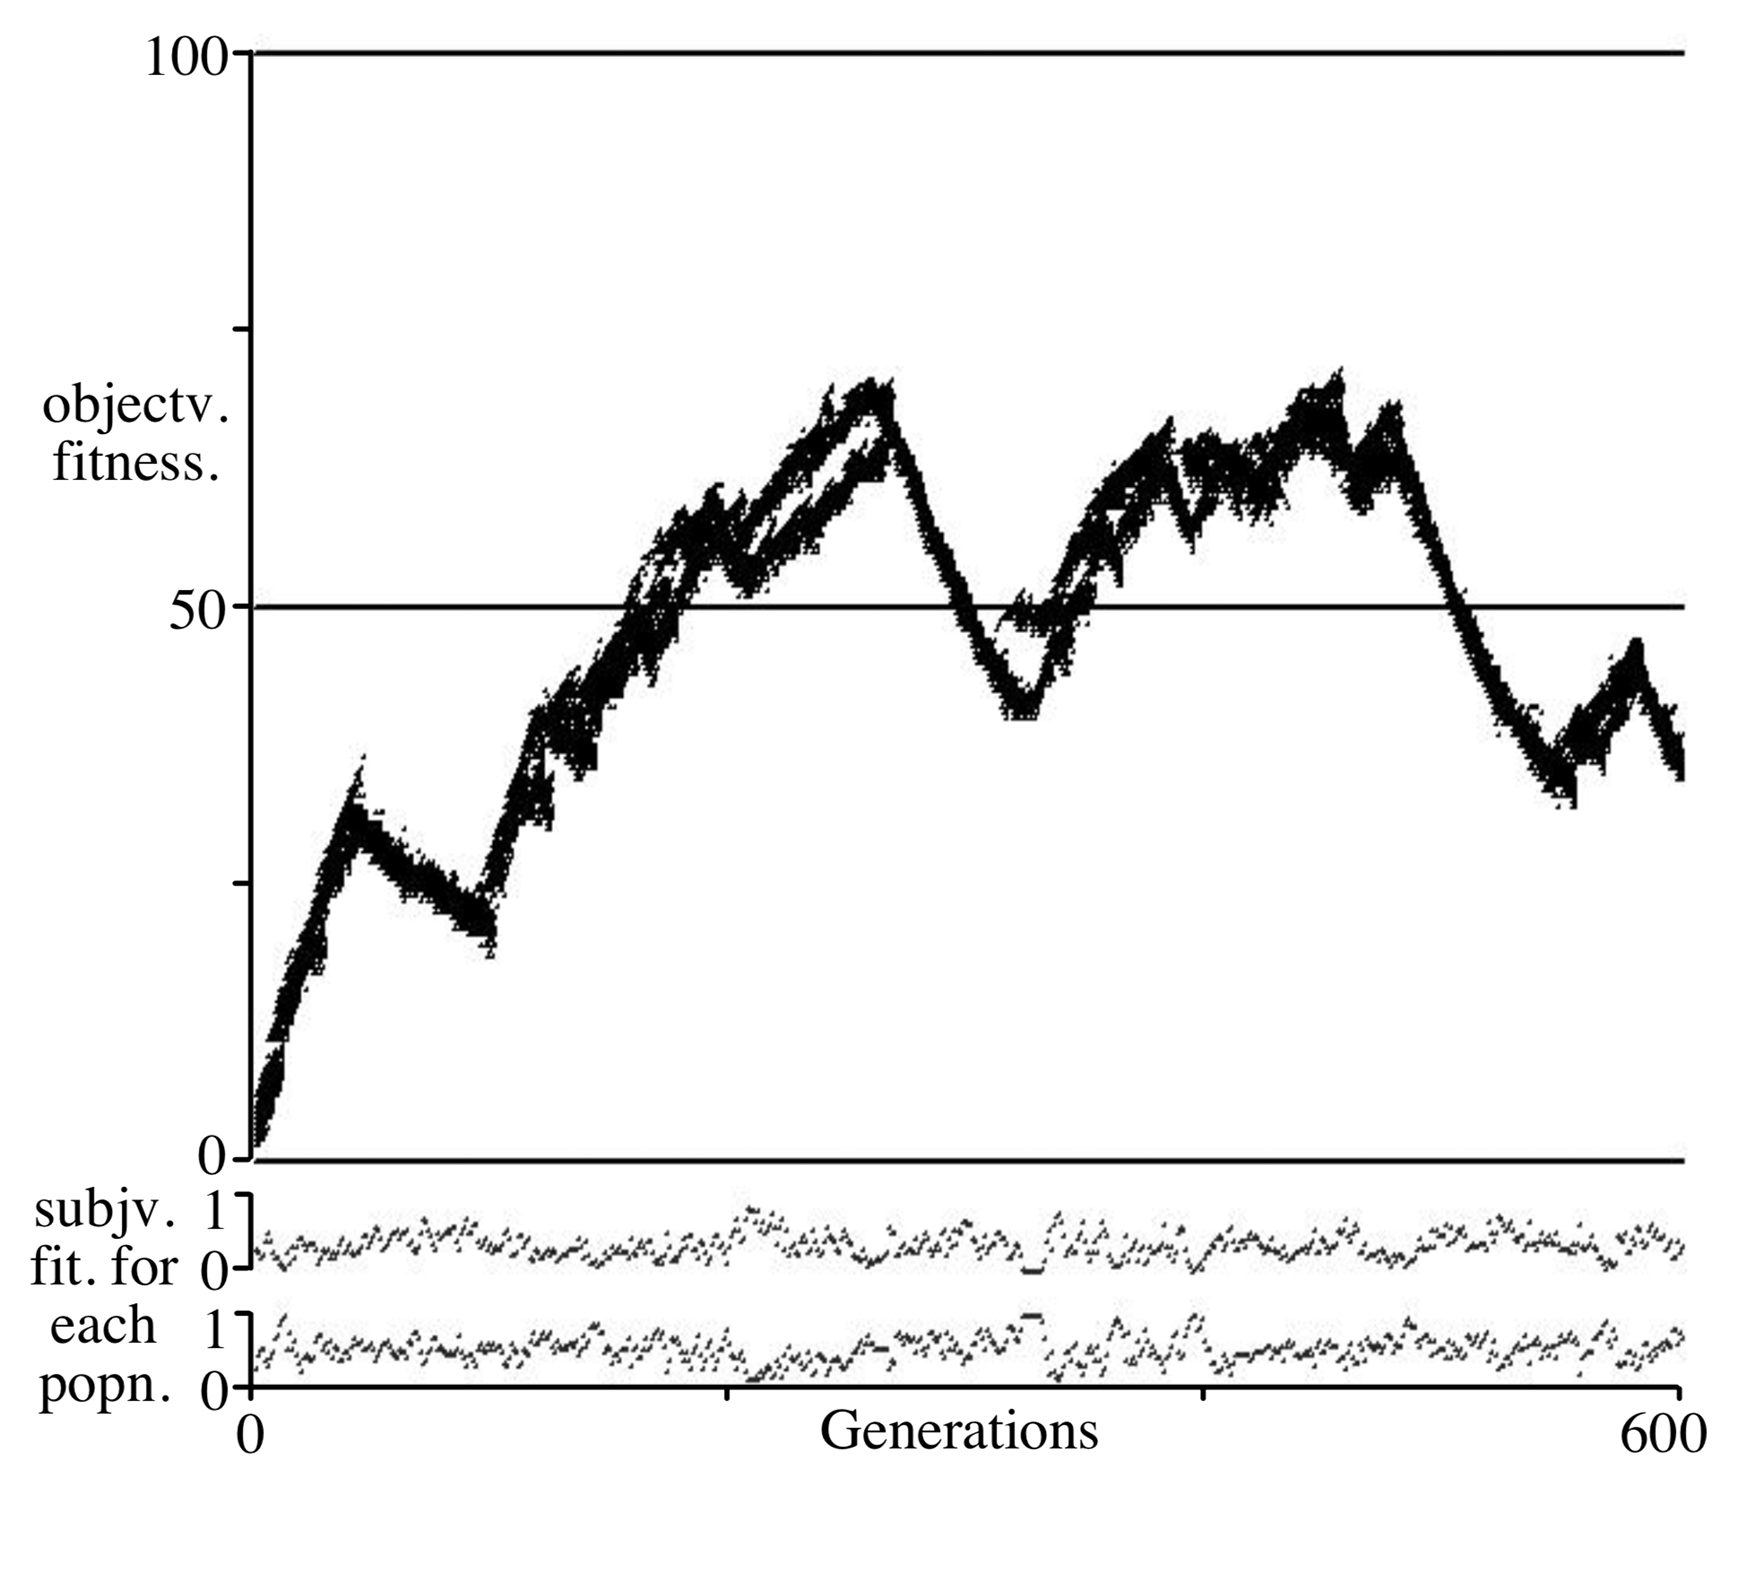
\includegraphics[height=6.5cm]{original/fig5.png}}
    \hspace{1.5mm}
    \subfloat[Reimplementation]{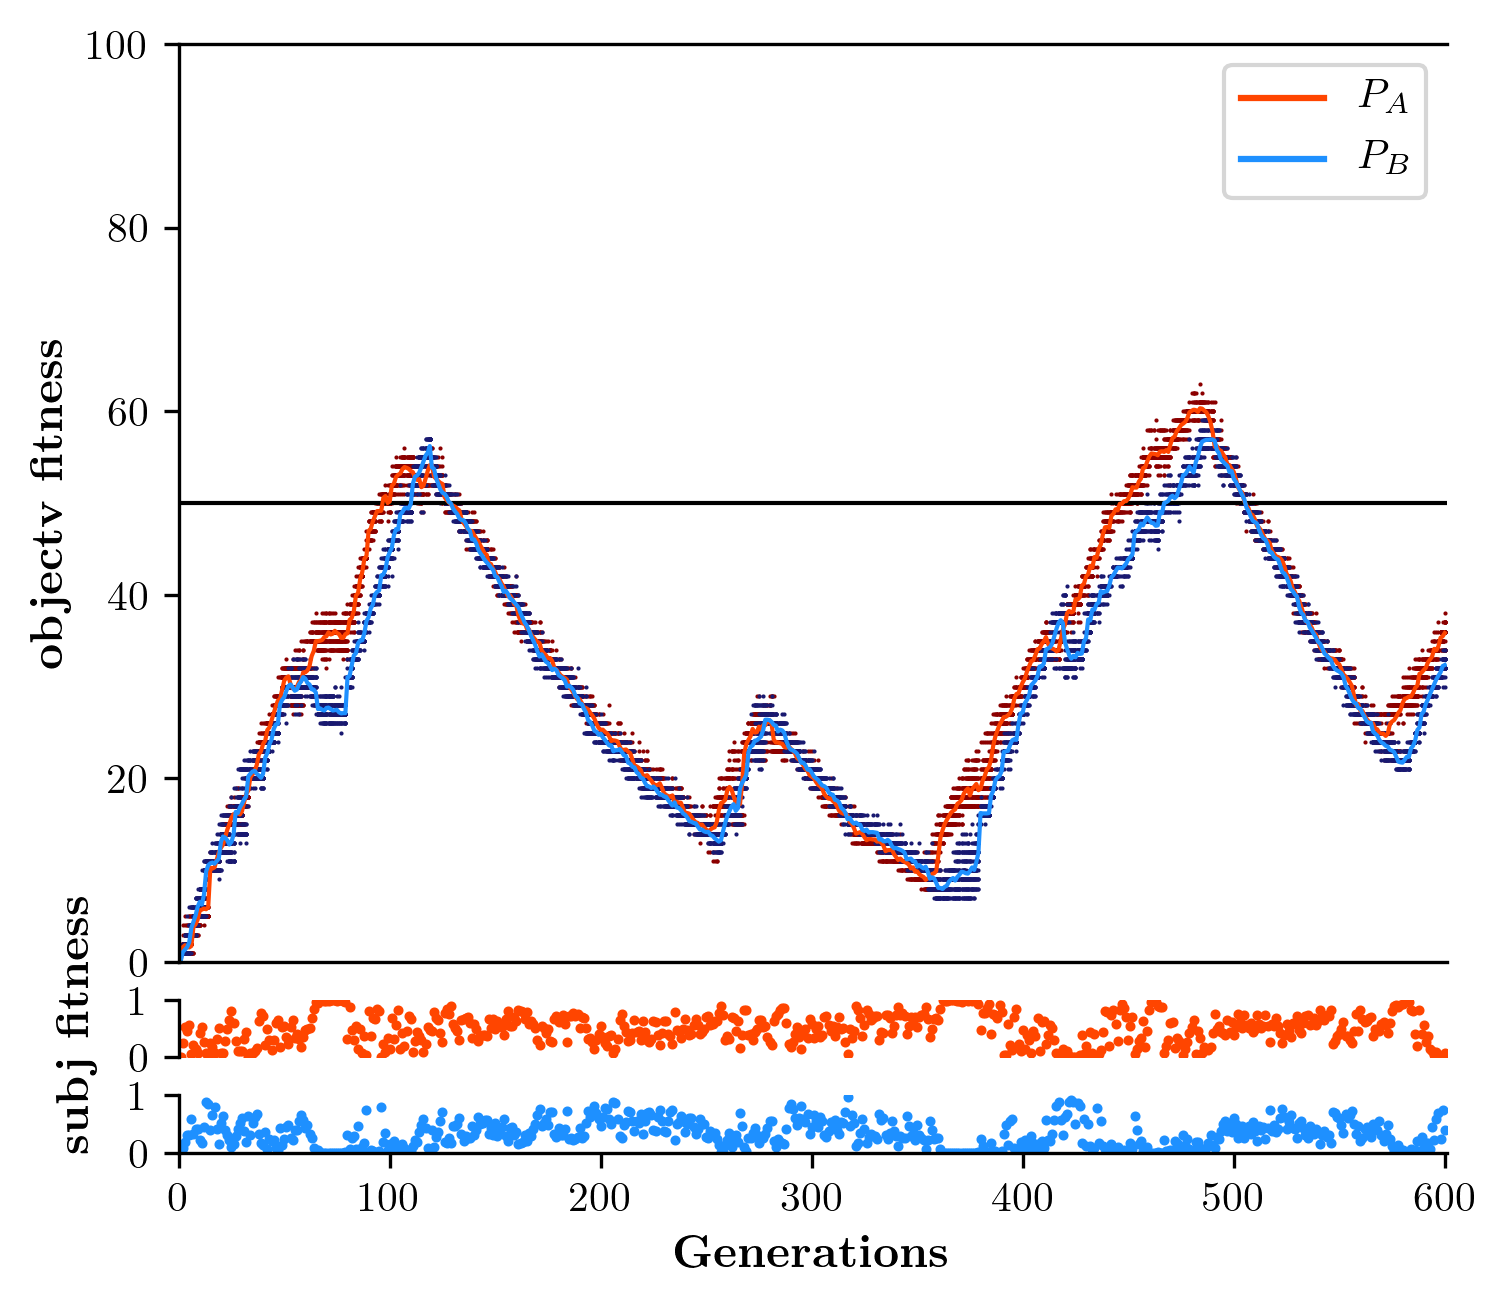
\includegraphics[height=6.5cm]{plots/fig5.png}}
    \end{tabular}
    \caption[]{$i=\{2,50\}$, intransitive=true \textit{(Originally Figure 5)}}
    \label{fig:figure_5}
\end{figure}



\section{Extension}
\noindent \textbf{Hypothesis:} Increasing diversity in populations during competitive coevolution can reduce the effects of relativism provided there is some selection pressure to improve. \\

\subsection{Description}
It is well accepted that high diversity in a population is key to avoiding premature convergence \parencite{Chong:2009}. Figure \ref{fig:figure_5} illustrates a scenario where there is reduced pressure to improve due to cyclic behaviour. When the population starts clustering into specialising on single traits the selective pressure to increase overall fitness is sabotaged by the subjective fitness assessment. If this cyclic behaviour can be mitigated or introduced in a less constant manner the selection pressure for higher values as defined by $a(d) > b(d)$ should have more weight. In other terms volatility should be introduced to the population to avoid premature convergence where progress is punished.\\

\noindent Two main ideas are explored to handle this: \textbf{reduced virulence} (RV) to maintain balance and \textbf{hall of fame} (HOF) to encourage long term progress. Brief summaries of the two follow.\\

\noindent \cite{Cartlidge:2004} proposes avoiding divergent behaviour by reducing virulence using the phantom parasite originally proposed by \cite{Rosin:1997}. This works by making subjective fitness a function of both the normal score and a virulence parameter $\lambda$ (see Equation \ref{eq:reduce_virulence}). Fundamentally, this equation will penalise those scoring higher than a fraction ($\lambda$) of the highest individual.
\begin{equation}
\label{eq:reduce_virulence}
    f(x, \lambda) = \frac{2x}{\lambda}-\frac{x^2}{\lambda^2}
\end{equation}
\noindent $\lambda$ can take any value however the three main values usually considered are: $1.0$ [Maximum Virulence], $0.75$ [Moderate Virulence] and $0.5$ [Null Virulence]. The original paper covers application of the concept to the counting ones domain using single trait individuals ($i=\{1,100\}$). Two modifications are made that complicate the domain: a bias is introduced for a single population that encourages 1 alleles during mutation and half points are awarded in $f_\text{subj}$ when $f_\text{obj}$ is equal for two individuals. This extension studies the effects of reducing virulence onto the multi-trait intransitive problem (Experiment 3) without these extra biases.\\

\noindent A hall of fame (HOF) can be considered as an extra population made up of individuals from previous generations, these are usually the best and are otherwise known as elites. These individuals can be incorporated into fitness functions to reduce the chances of `forgetting' and drive progress \parencite{Ranjeet:2011}.\\

\noindent Also touched upon are the drawbacks of using fitness proportionate selection (FPS) due to it encouraging proliferation of individuals that have a much higher fitness than the rest of the population \parencite{Blickle:1996}. Both tournament selection (TS) and stochastic universal sampling (SUS) are considered as alternatives. SUS as it avoids over selection of high fitness individuals due to noise (a dominant individual will at most only get selected one extra time than it should) \parencite{Blickle:1996}. Along with TS as when using a small tournament size, e.g. 3, lower probability elements have a high probability of being selected.


\subsection{Implementation}
\noindent Virulence was implemented as a wrapper for the selection method, where the fitness values are modified before being passed to the test selection method (e.g. FPS, SUS, TS). Fitness values were first normalised across each population between 0 and 1 before applying Equation \ref{eq:reduce_virulence}.\\

\noindent The HOF method captures a rolling window of elites for the last $|H|$ generations and then uses a random sample of ($S_H$) in conjunction with Equation \ref{eq:scoring}. \cite{Rosin:1997} suggests random sampling is preferable as usually the computational effort to maintain performance information is not worth it. In an ideal world the elites picked for the HOF ($H$) would be based on $f_\text{obj}$, however with the intention of not introducing potentially undefinable information into the selection, $f_\text{subj}$ is used. The downside of this is that relativism is likely still going to be present in the system. A HOF is only used where stated.\\

\noindent The selections methods implementations are based on pseudo-code from \cite{Blickle:1996}.

\subsection{Results}
\noindent The following results are described in the order that experimentation occurred. Initially targeting reduced virulence, introducing new selection methods and then incorporating a hall of fame. Note that all plots regarding the extension were created using the same random seed so all differences stem from the modifications introduced. Contrasts are made against Figure \ref{fig:figure_5} from the base experiment.\\


\noindent Starting with Figure \ref{fig:ext_virulence} the results of incorporating reduced virulence can be seen for two values of $\lambda$: 0.5 and 0.75. The effects of null virulence are clear from Figure \ref{fig:ext_virulence_0.5}, there is little selection pressure, meaning little incentive to move away from the mutual bias position once it is reached. Although this stops steep dives like in Experiment 3, there is not enough incentive for progress in the objective metric. Conversely, 0.75 yielded little if any improvement in regards to stability, however the overall max objective reached was higher 78 vs 64. An assumption was made that a more stable selection method may mitigate this.

\begin{figure}[H]
    \centering
    \begin{tabular}{cc}
    \subfloat[$\lambda=0.5$\label{fig:ext_virulence_0.5}]{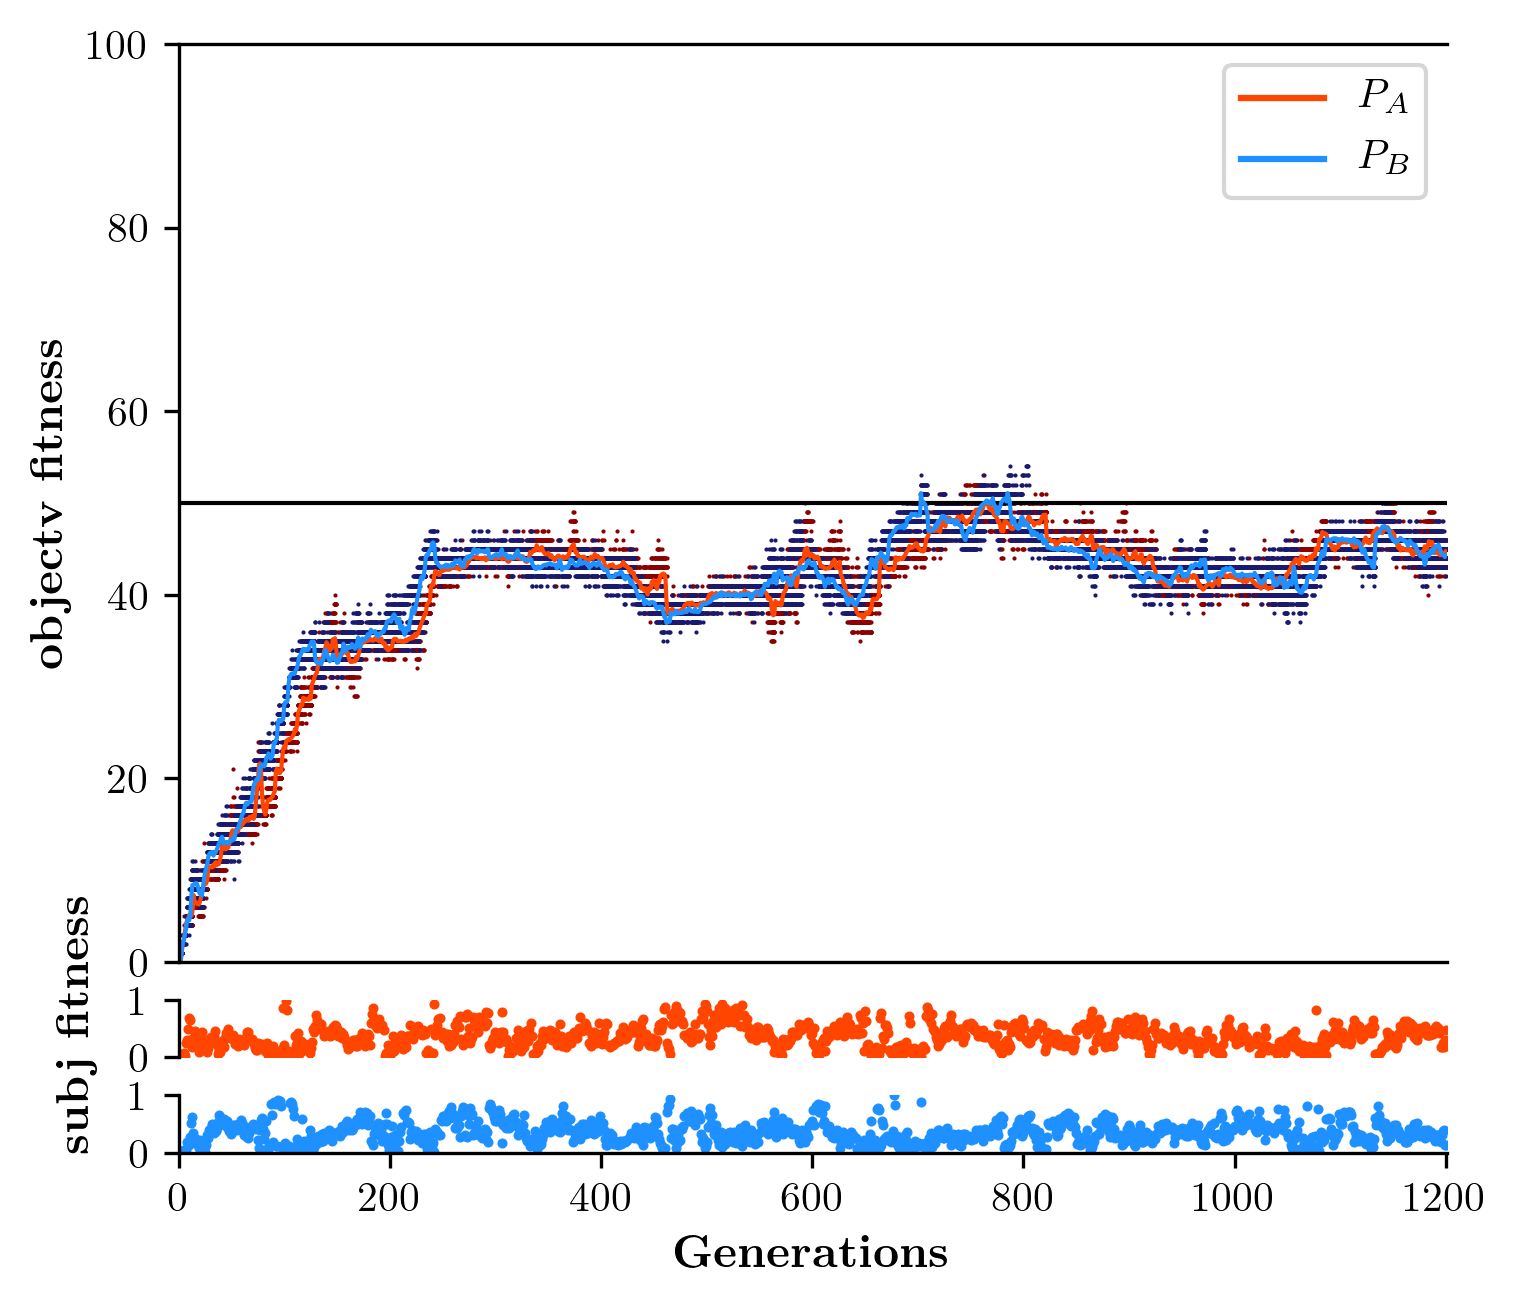
\includegraphics[height=6.5cm]{plots/fig_5_v0.5.png}}
    \hspace{1.5mm}
    \subfloat[$\lambda=0.75$\label{fig:ext_virulence_0.75}]{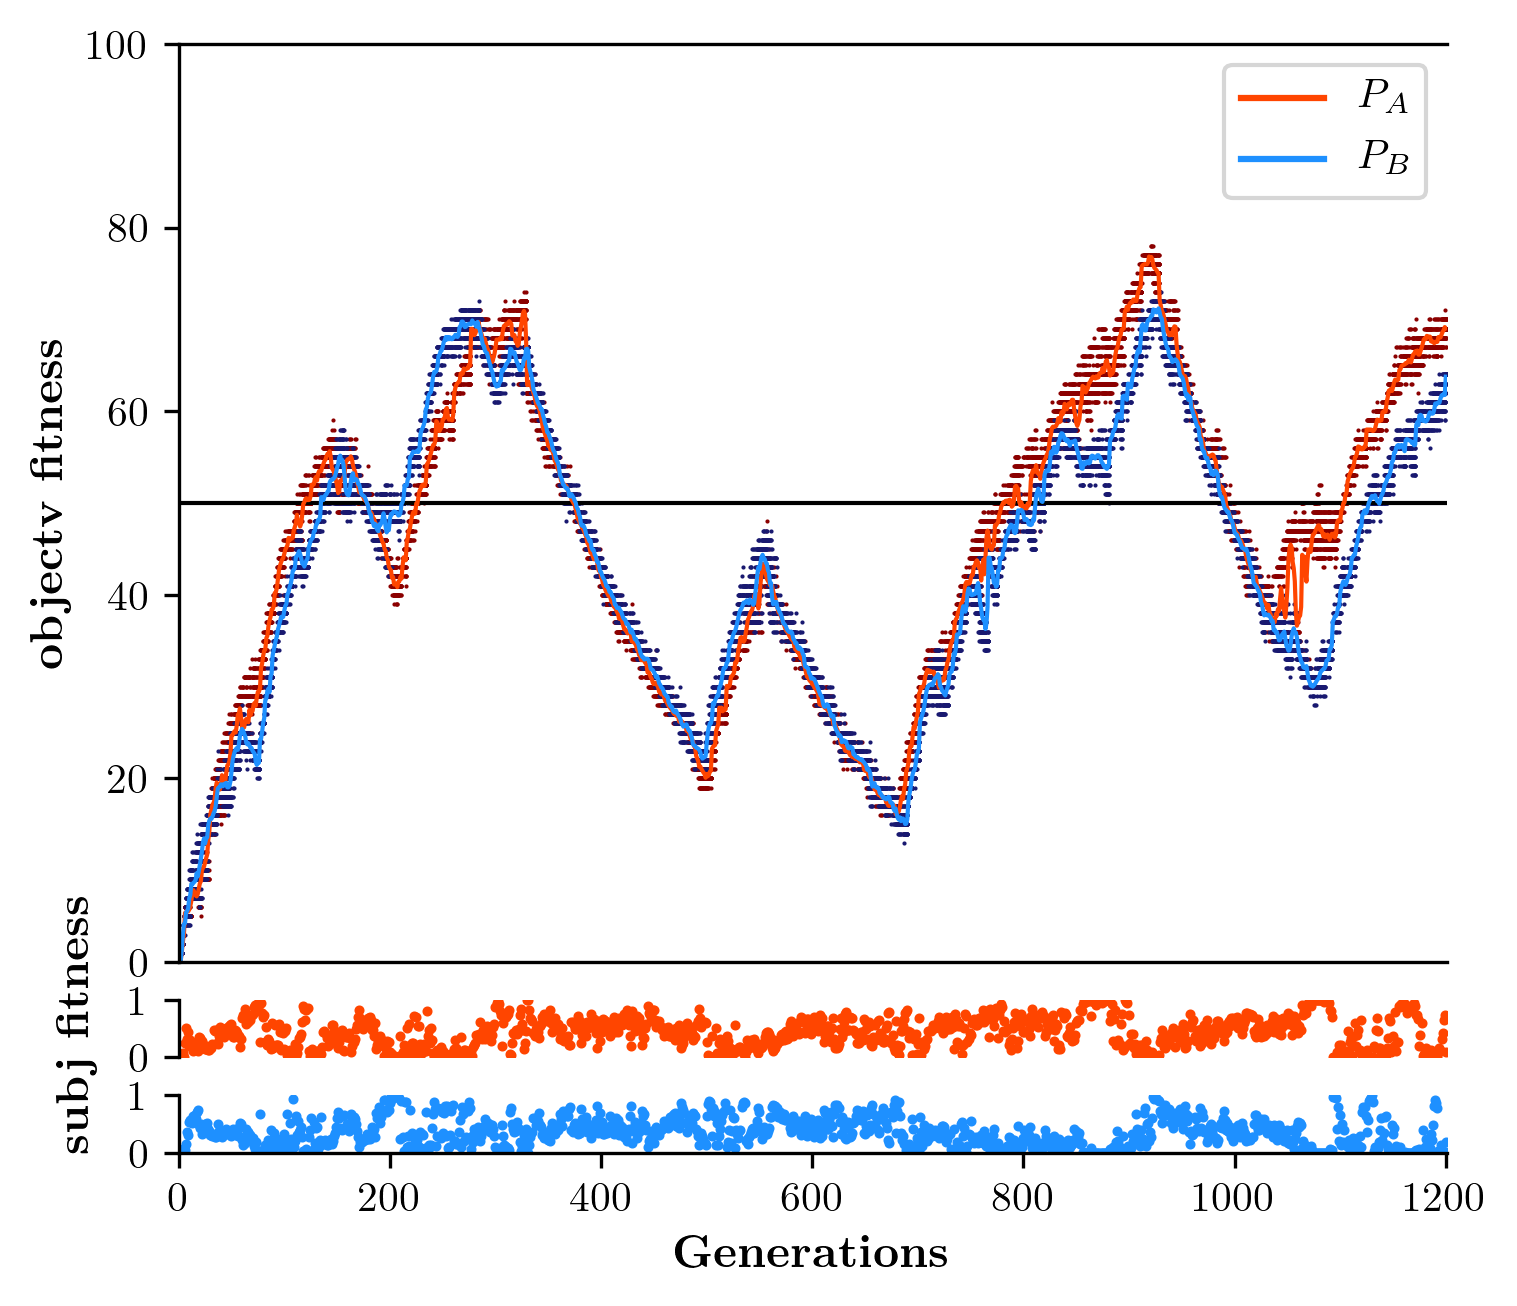
\includegraphics[height=6.5cm]{plots/fig_5_v0.75.png}}
    \end{tabular}
    \caption{$i=\{2,50\}$, intransitive=true\\Demonstration of different lambda values used for virulence reduction.}
    \label{fig:ext_virulence}
\end{figure}

\noindent The results of applying TS and SUS alongside RV with $\lambda=0.75$ can be seen in Figure \ref{fig:ext_selection}. It is clear that TS causes a high level of instability in the evolution with more frequent periods of shorter descent; this is also at the expense of a high objective score. On the other hand SUS starts exhibiting good behaviour, with generation 200 onwards staying at a consistent level above the mutation bias point; this indicates each individual is able to keep a constant pressure on maintaining both traits. As new generations are not able to be suddenly dominated by one lucky individual, a period of stability can occur all whilst enjoying the benefits of a more diverse population.

\begin{figure}[H]
    \centering
    \begin{tabular}{cc}
        \subfloat[TS ($n=3$)]{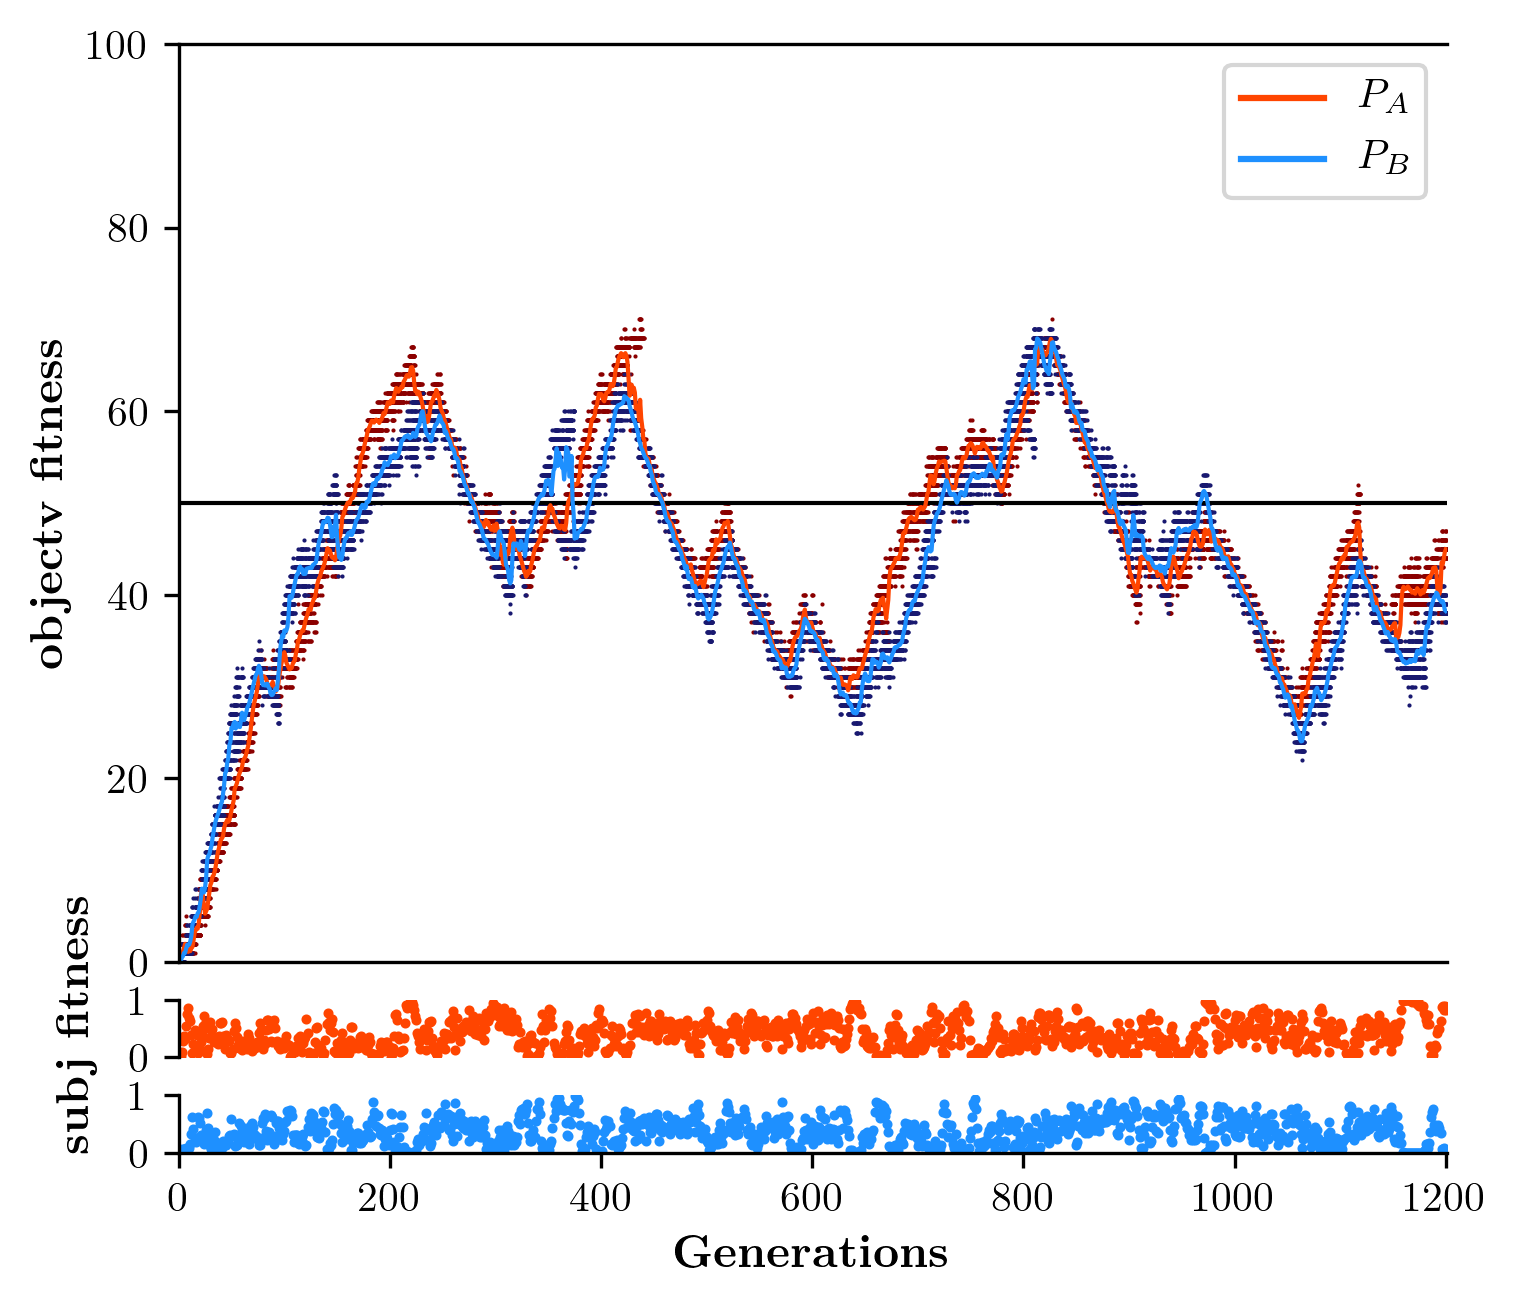
\includegraphics[height=6.5cm]{plots/fig_5_v0.75_ts.png}}
        \hspace{1.5mm}
        \subfloat[SUS\label{fig:ext_selection_sus}]{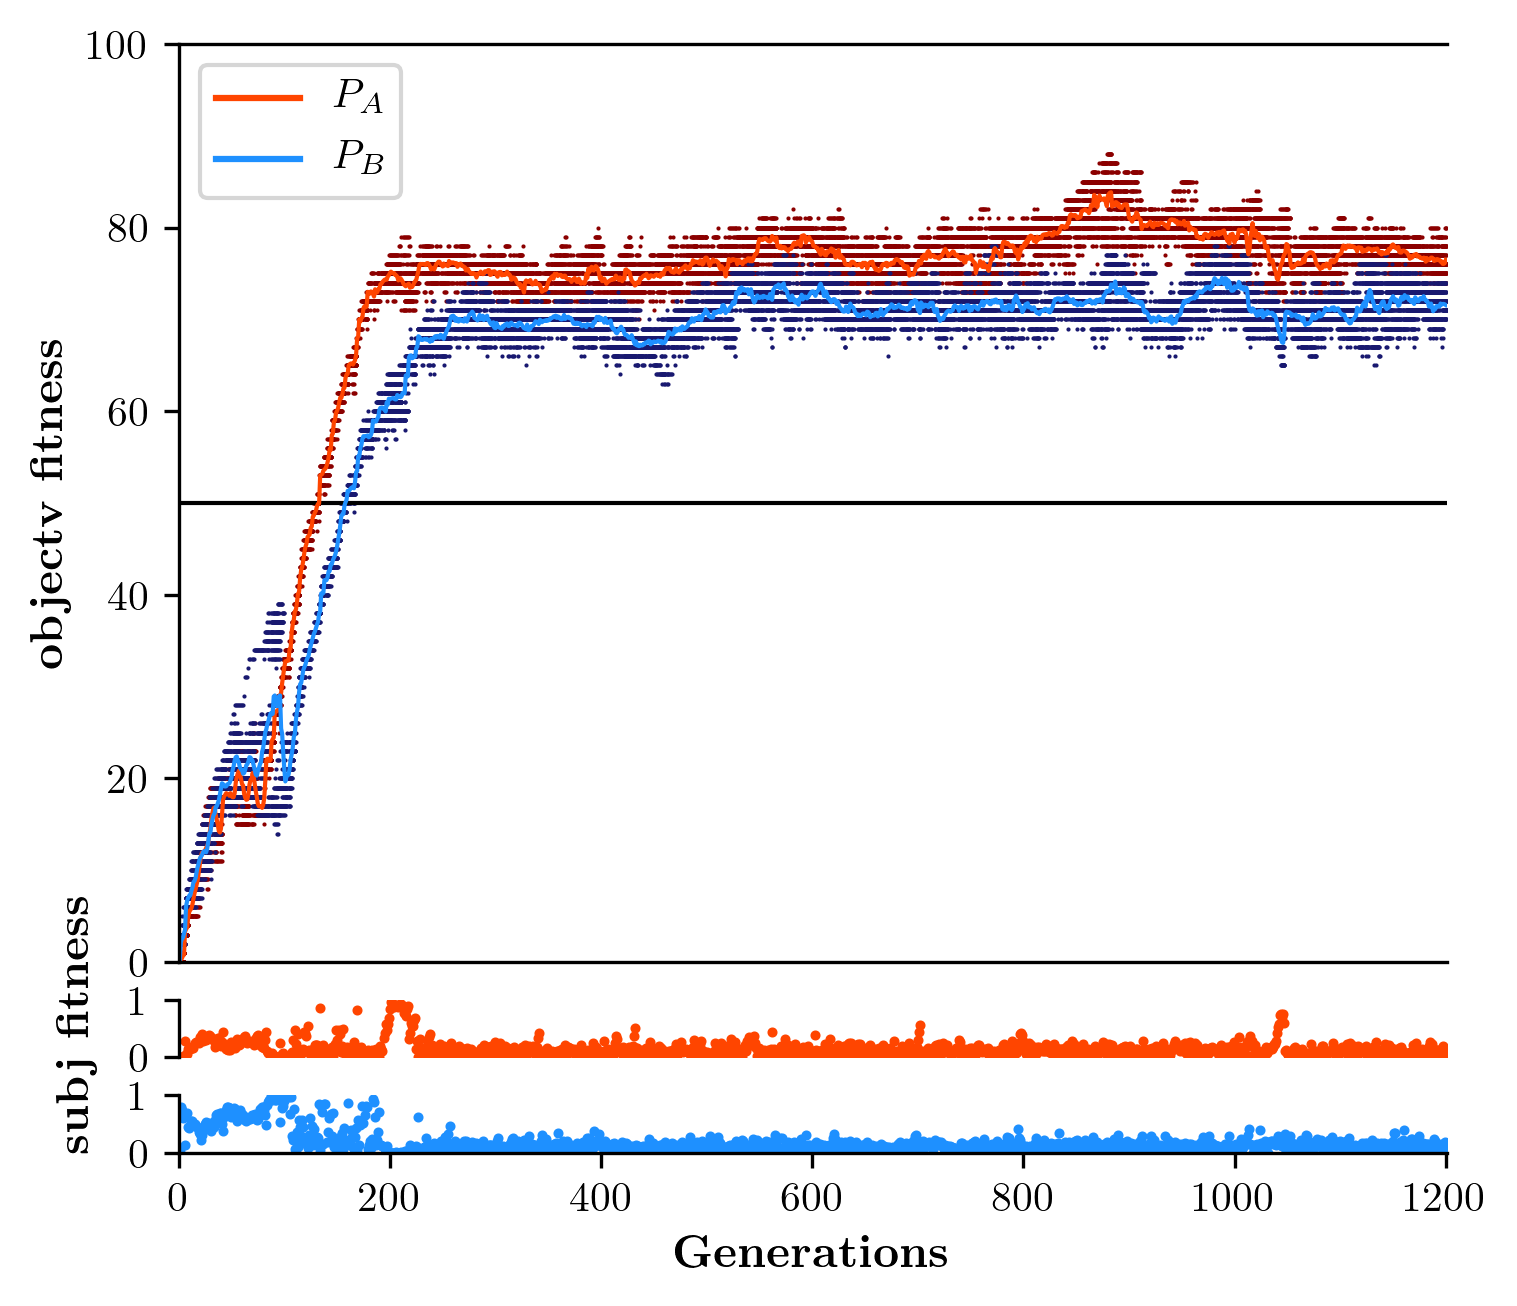
\includegraphics[height=6.5cm]{plots/fig_5_v0.75_sus.png}}
    \end{tabular}
    \caption{$i=\{2,50\}$, intransitive=true, $\lambda=0.75$\\Demonstration of different selection techniques with reduced virulence.}
    \label{fig:ext_selection}
\end{figure}

\noindent The final addition is the introduction of HOF. Figure \ref{fig:ext_hof_only} is provided in the appendix as a control -- it shows that although HOF increases the overall objective it does not provide the diversity maintenance required to stop relativism causing downward spikes. Figure \ref{fig:ext_hof} shows what happens when reduced virulence provides this required mechanism. Figure \ref{fig:ext_0.75_hof_sus} is a natural progression from Figure \ref{fig:ext_selection_sus} with HOF added on top of SUS. The ability to now reach high objective values of 90-100 is present however there is large inter-population noise; the reason for this is unknown but could be attributed to HOF implementation making use of the selected selection method -- i.e. the HOF implementation may just work better with FPS. Taking away SUS and leaving just HOF and VS gives the best result. Although there is occasional drops the high diversity gives a high chance of the populations re-engaging competitively as opposed to cooperatively. Notably adding HOF for $\lambda=0.5$ (plot not shown), causes the average objective fitness to rise above 50; this is likely because once a good subset of previous generations is available it becomes the new neutral point.

\begin{figure}[H]
    \centering
    \begin{tabular}{cc}
        \subfloat[HOF + SUS\label{fig:ext_0.75_hof_sus}]{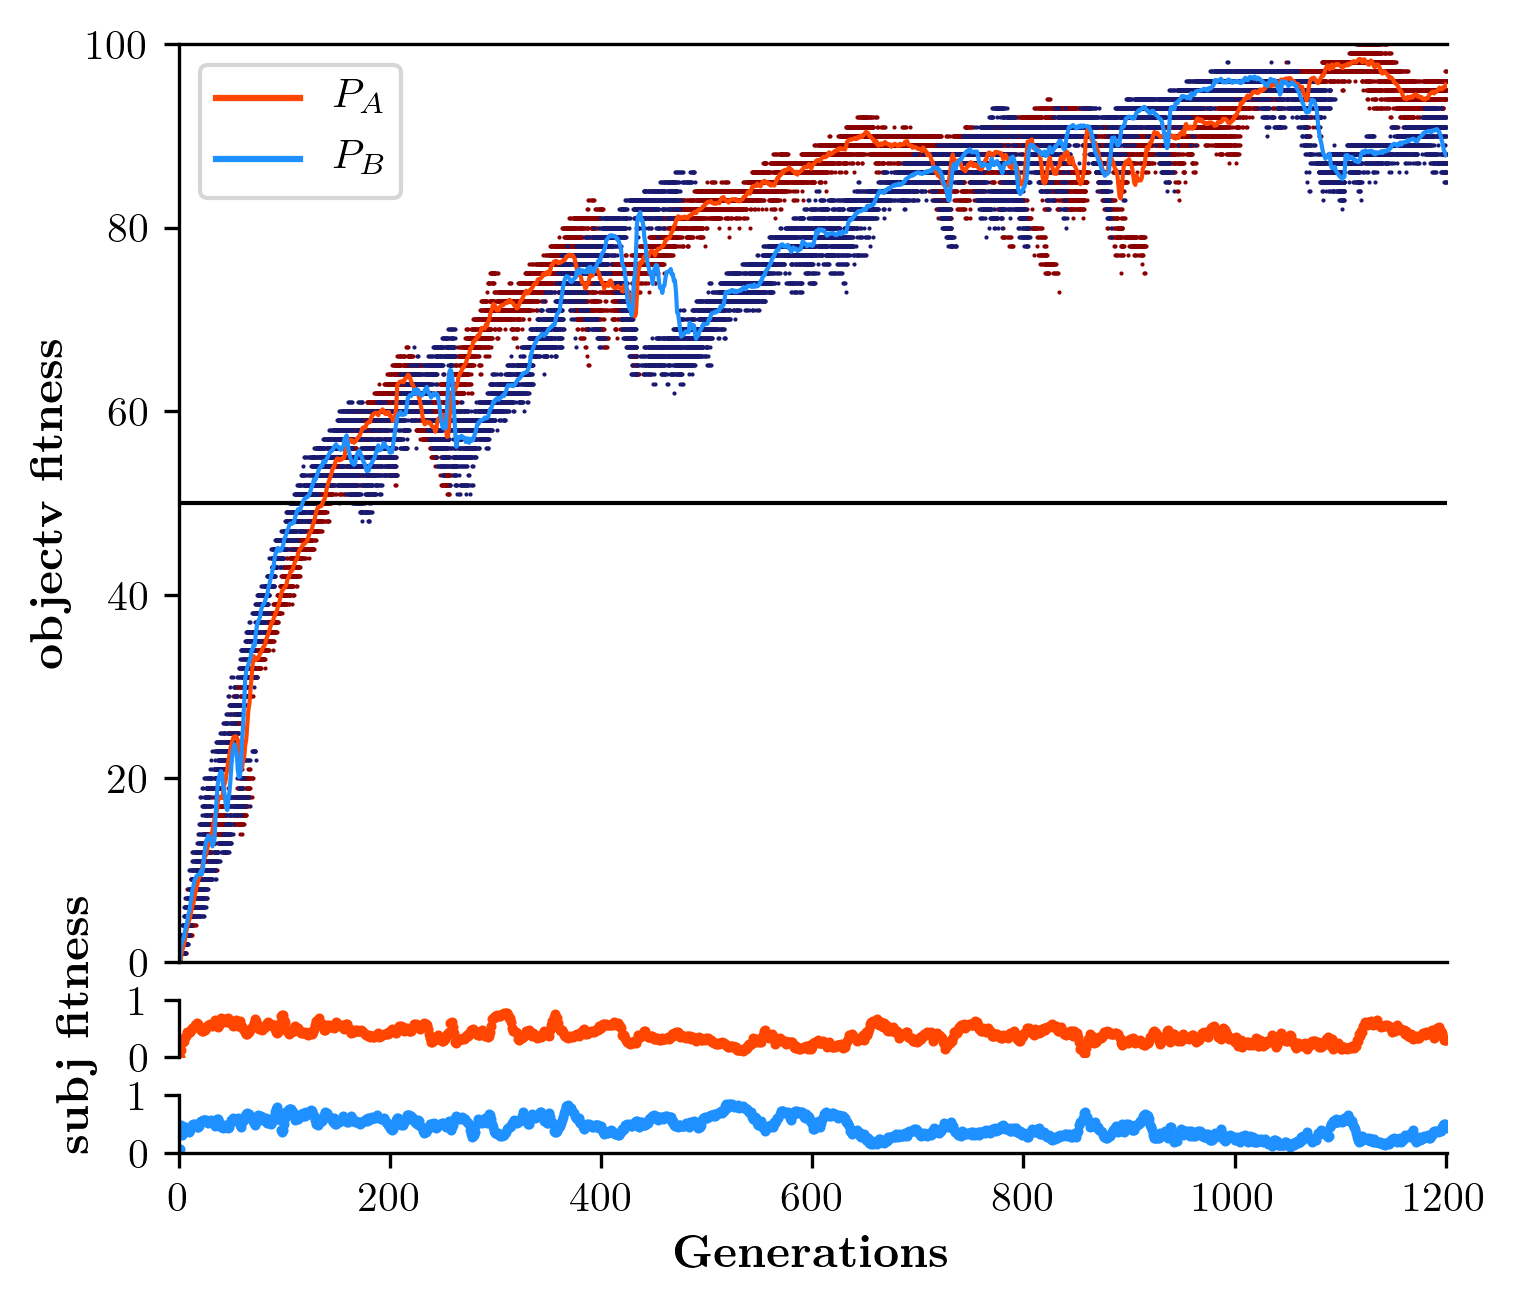
\includegraphics[height=6.5cm]{plots/fig_5_v0.75_sus_hof.png}}
        \hspace{1.5mm}
        \subfloat[HOF\label{fig:ext_0.75_hof}]{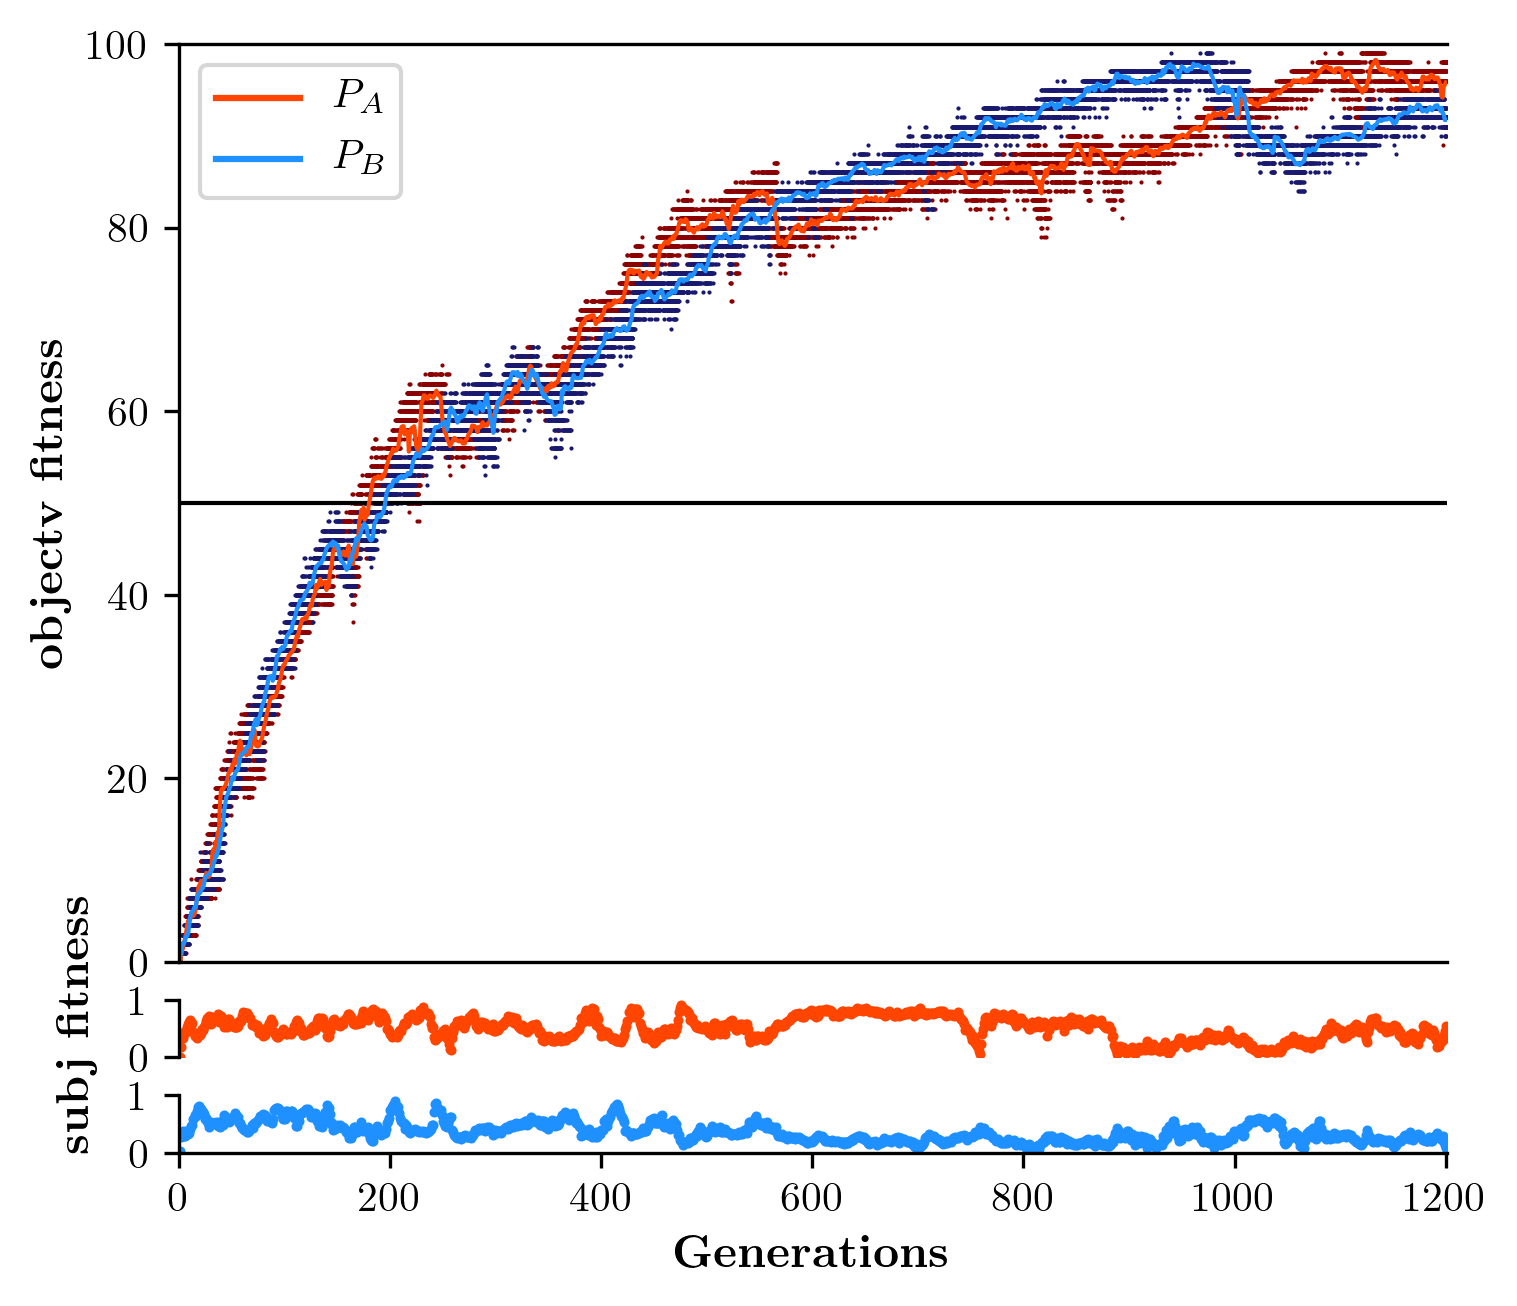
\includegraphics[height=6.5cm]{plots/fig_5_v0.75_hof.png}}
    \end{tabular}
    \caption{$i=\{2,50\}$, intransitive=true, $|H|=50$, $S_H=10$, $\lambda=0.75$\\ Demonstration of hall of fame (HOF) introduction alongside reduced virulence.}
    \label{fig:ext_hof}
\end{figure}

\section{Conclusion}
This paper started by reimplementing the work of \cite{Watson:2001} to demonstrate potential failings that may affect a coevolution GA. The implementation was verified against the original work to allow further exploration of the problem domain.\\

\noindent The problem was posed of reducing the effects of relativism through diversity. It was found that using a combination of mechanisms, one to drive diversity and one to ensure progress was being made that indeed the effects could be partially mitigated. However, in the punitive problem studied, it was not possible to completely avoid drift towards the mutation bias and potentially below. This suggests that in some scenarios the subjective scoring function may just be too contradictory to blindly trust a coevolutionary setup. That being said, the clear trend for higher values and rapid recovery from downward trajectory satisfies the hypothesis. Note that not one of the added mechanics could fix the problem by itself: either RV + HOF or RV + SUS was required for a reasonable improvement to be made.\\

\noindent There are many areas that can be expanded on to further understand the results shown and increase confidence. These should cover: optimisation of the many parameters controlling the mechanisms, trials of more complex HOF systems, such as those demonstrated by \cite{Nogueira:2013}, and more detailed focus on the individuals make-up to verify if the expected distribution of trait values are present. Branching from this, individuals are currently only considered with two traits, the ideas proposed may fail when more are introduced due to even more tight binding from the intransitive relationships.


\printbibliography

\newpage
\begin{appendices}
\section{Extra Figures}
\begin{figure}[H]
    \centering
    \begin{tabular}{cc}
    \subfloat[Original \parencite{Watson:2001}]{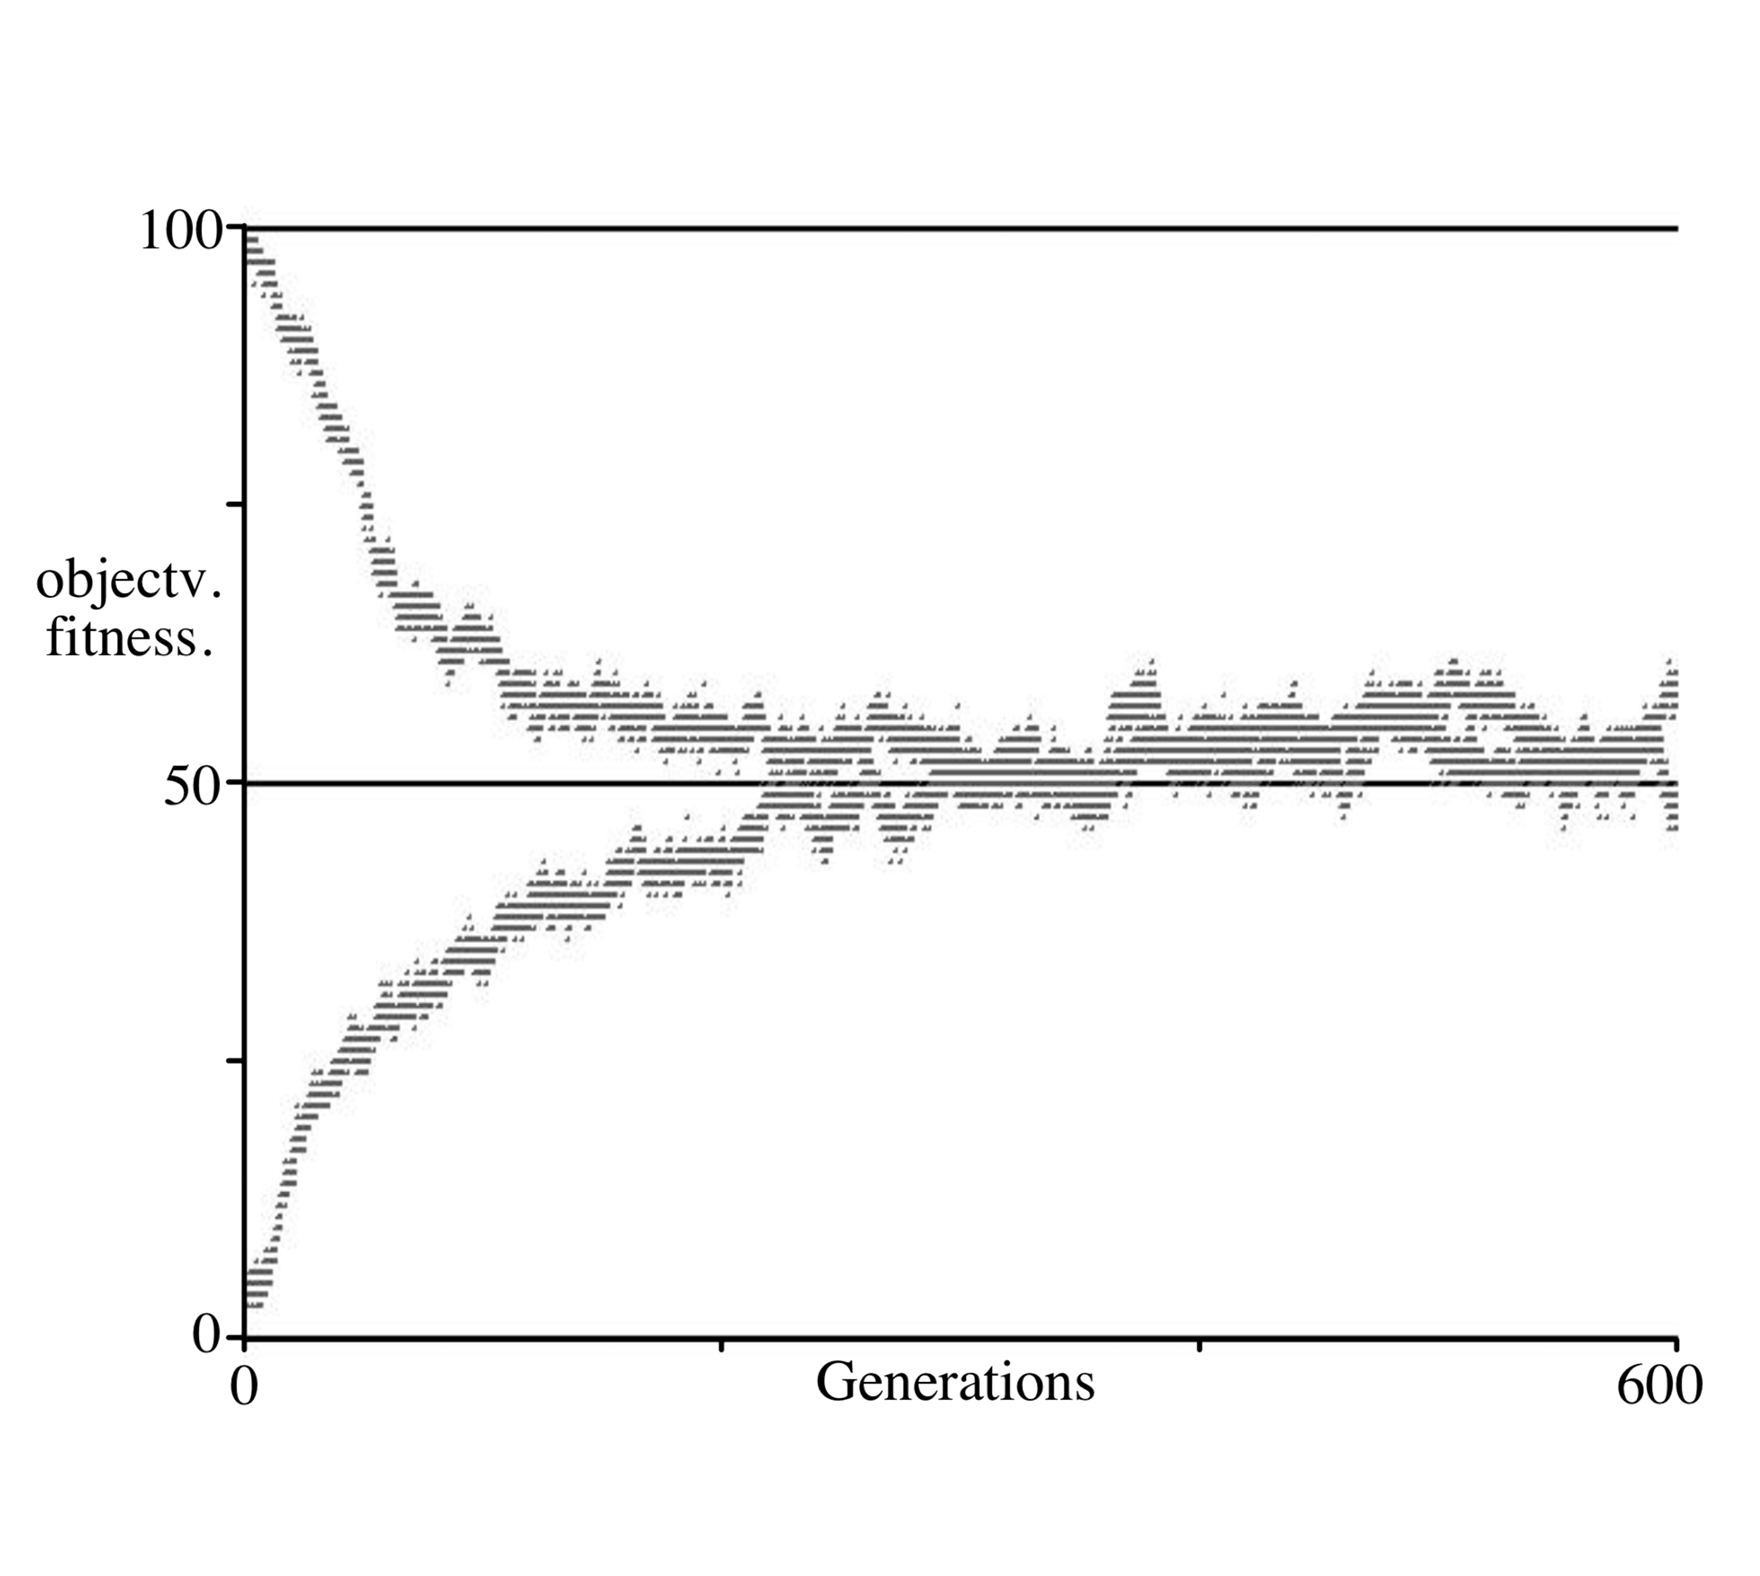
\includegraphics[height=6.5cm]{original/fig1.png}}
    \hspace{1.5mm}
    \subfloat[Reimplementation]{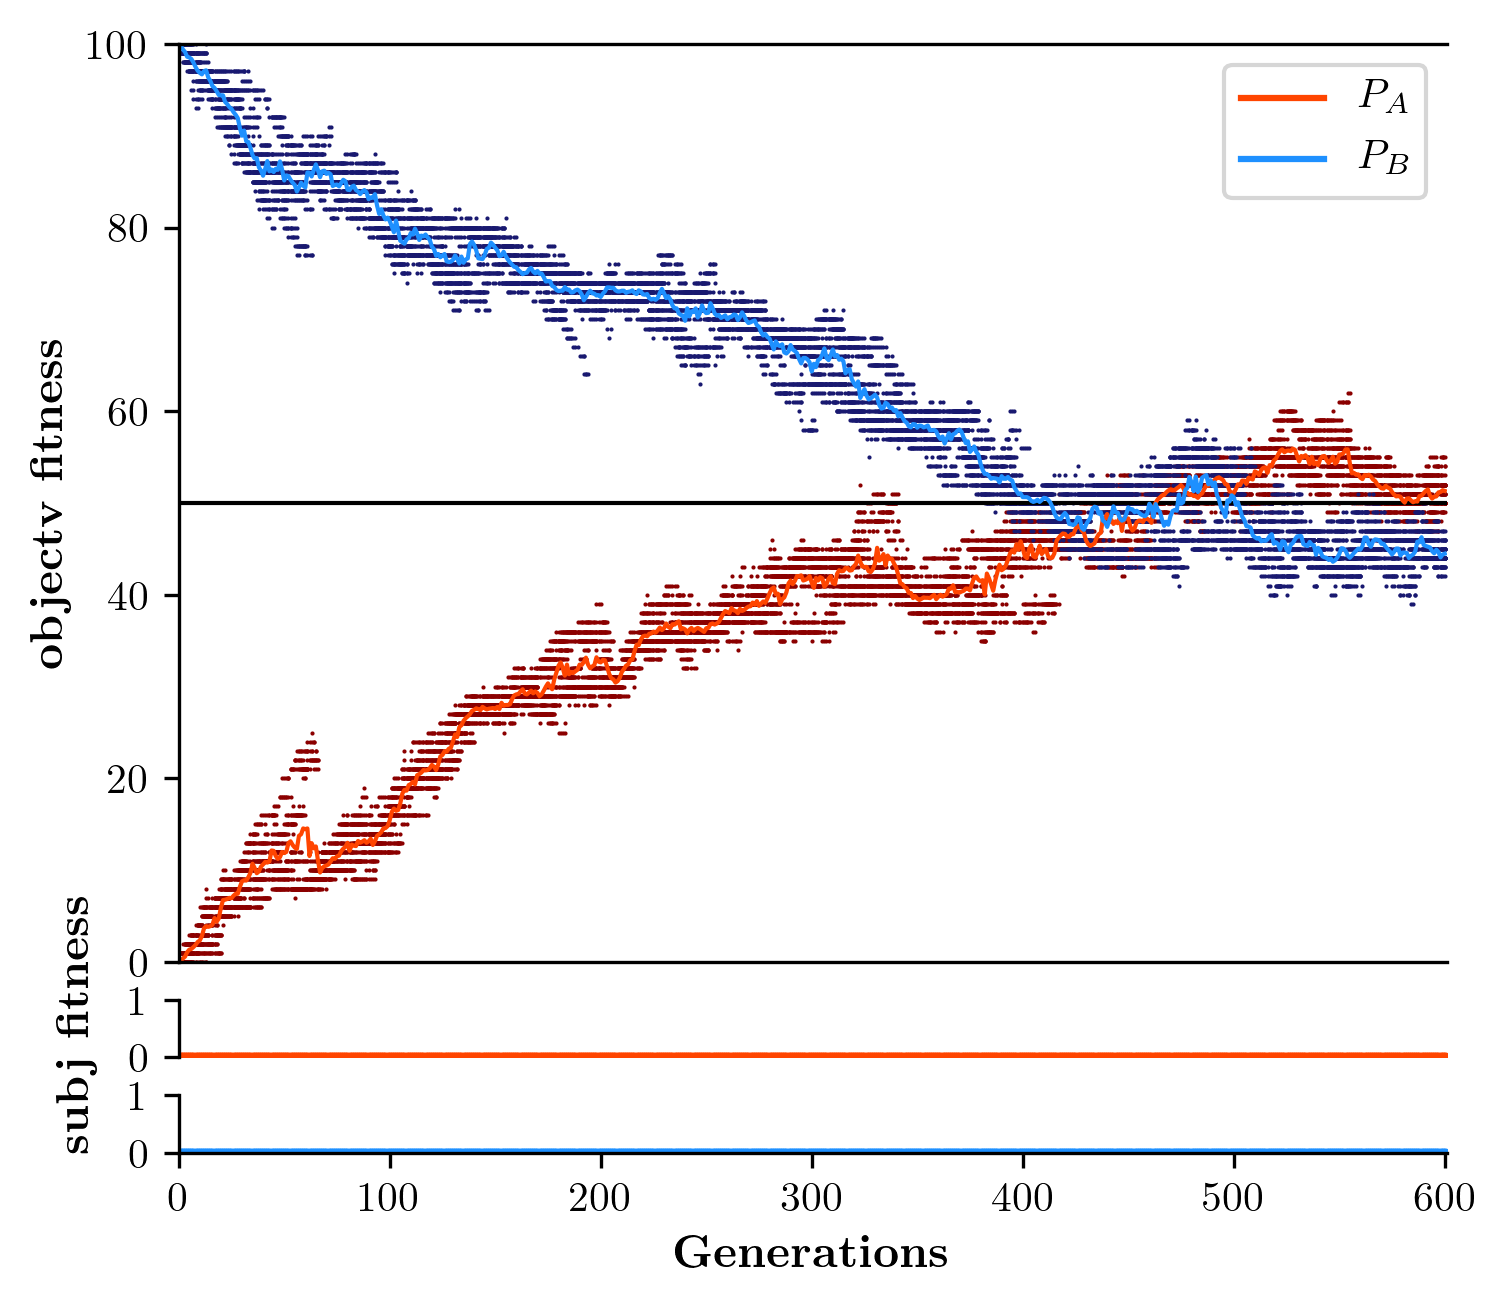
\includegraphics[height=6.5cm]{plots/fig1.png}}
    \end{tabular}
    \caption{$i=\{1,100\}$ Control figure where $f_\text{subj}=0$ (no scoring function) demonstrating natural drift to $t_l / 2 = 50$ due to mutation bias. \textit{(Originally Figure 1)}}
    \label{fig:figure_1}
\end{figure}
\begin{figure}[H]
    \centering
    \begin{tabular}{cc}
    \subfloat[Original \parencite{Watson:2001}]{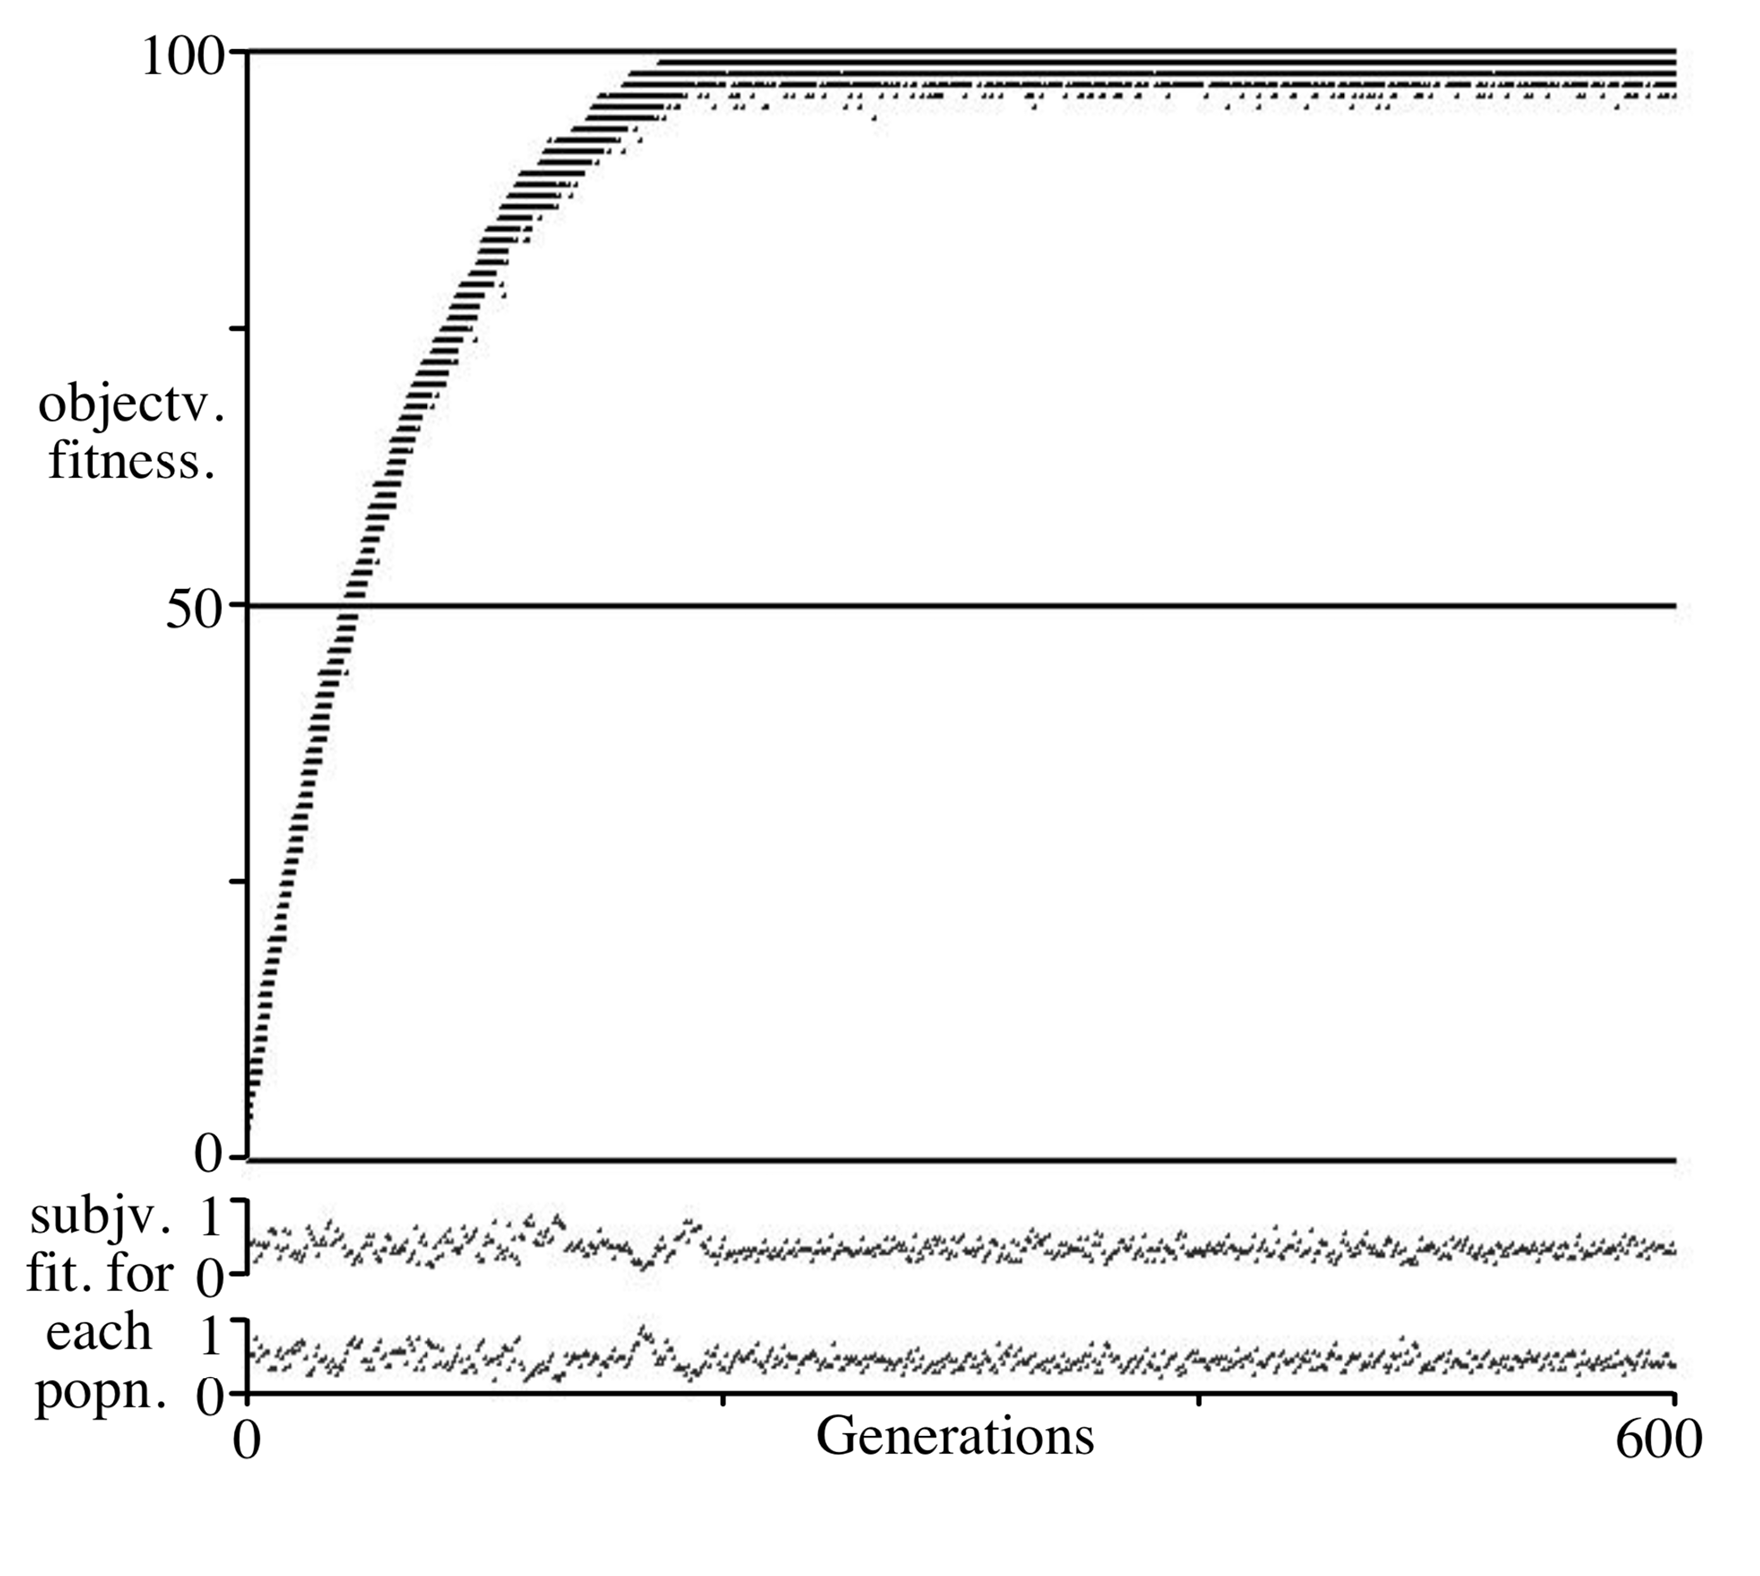
\includegraphics[height=6.5cm]{original/fig2.png}}
    \hspace{1.5mm}
    \subfloat[Reimplementation]{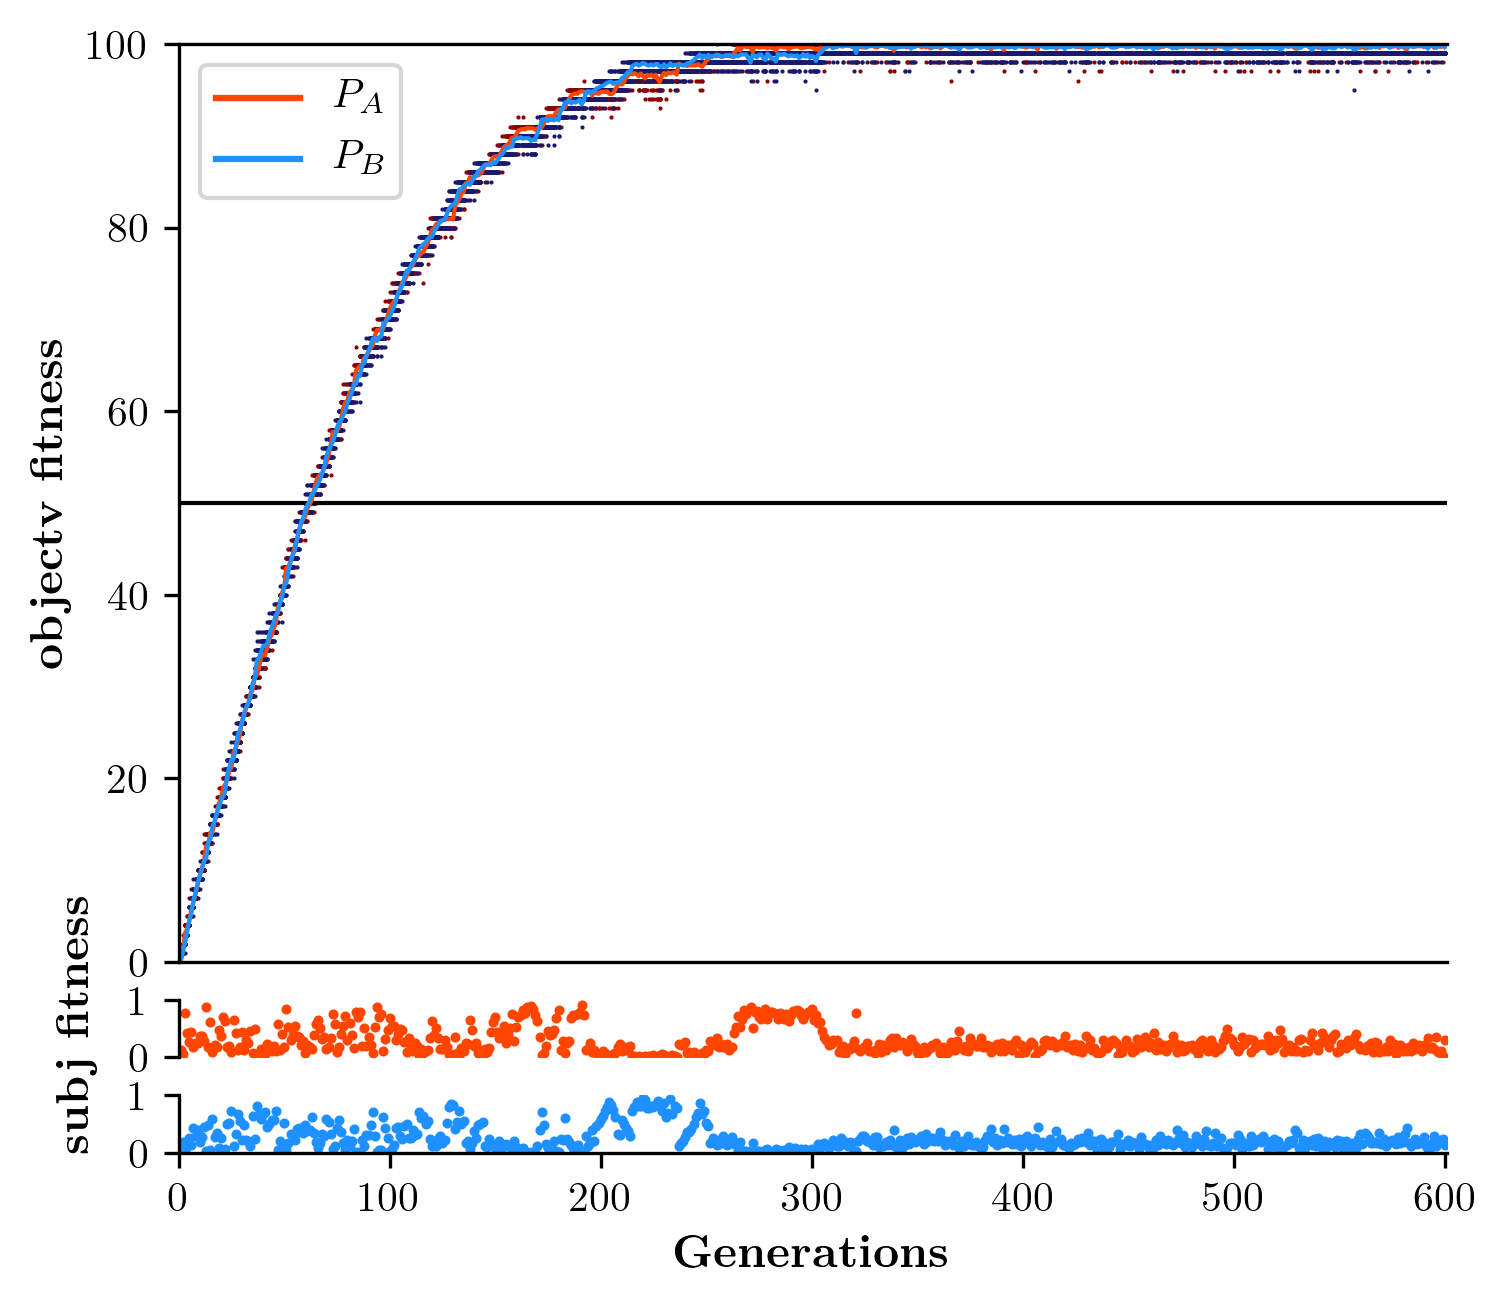
\includegraphics[height=6.5cm]{plots/fig2.png}}
    \end{tabular}
    \caption{$i=\{1,100\}$ Control figure showing GA working in ideal conditions. \textit{(Originally Figure 2)}}
    \label{fig:figure_2}
\end{figure}

\begin{figure}[H]
    \centering
    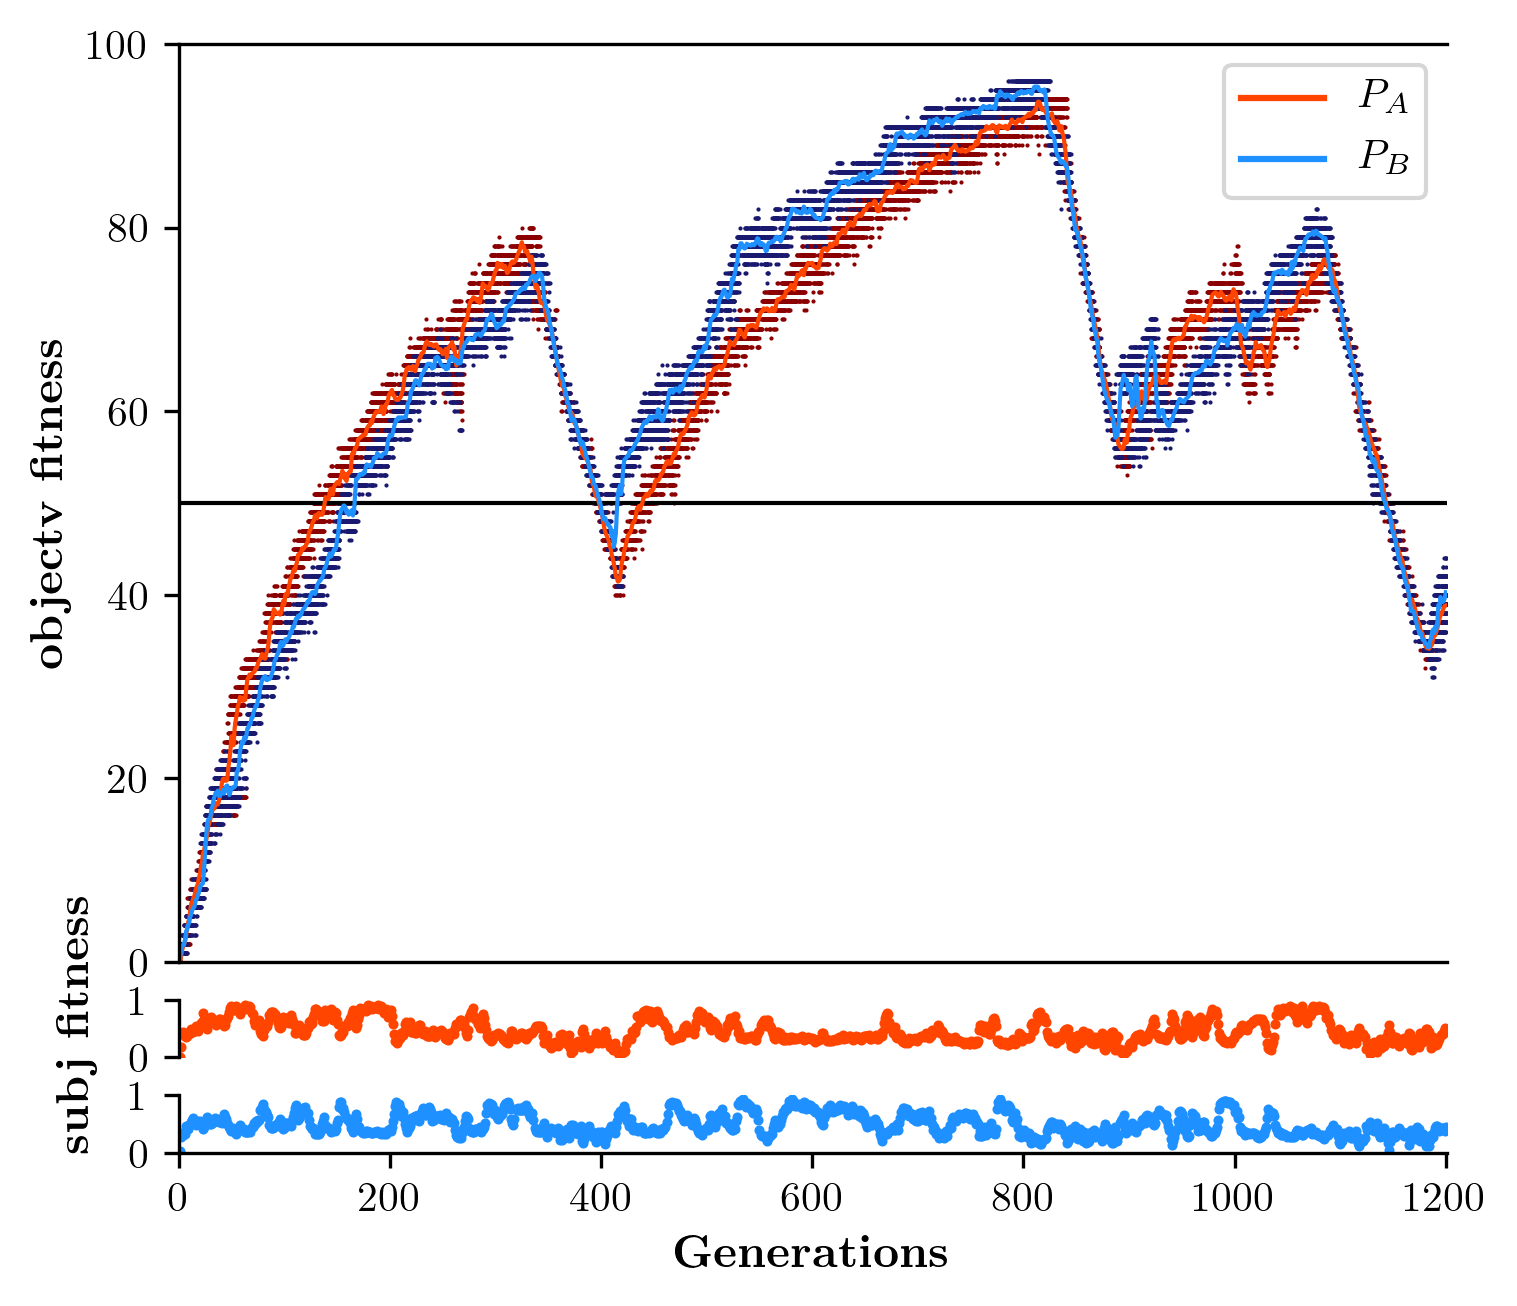
\includegraphics[height=6.5cm]{plots/fig_5_hof.png}
    \caption{$i=\{2,50\}$ intransitive=true, $|H|=50$, $S_H=10$}
    \label{fig:ext_hof_only}
\end{figure}


\newpage
\section{Code Listings}
\label{sec:codebase}
\subsection{assignment2.py}
\inputminted{python}{../code/assignment2.py}\newpage
\subsection{coevolution.py}
\inputminted{python}{../code/coevolution.py}\newpage
\subsection{representation.py}
\inputminted{python}{../code/representation.py}\newpage
\subsection{mutation.py}
\inputminted{python}{../code/mutation.py}\newpage
\subsection{scoring.py}
\inputminted{python}{../code/scoring.py}\newpage
\subsection{selection.py}
\inputminted{python}{../code/selection.py}\newpage
\subsection{plot.py}
\inputminted{python}{../code/plot.py}\newpage
\subsection{utils.py}
\inputminted{python}{../code/utils.py}\newpage


\end{appendices}



\end{document}